\documentclass[a4paper]{oblivoir}
\author{Moon Il-chul \\ \href{mailto:icmoon@kaist.ac.kr}{icmoon@kaist.ac.kr} 
   \and Ryu Jae-hyeon
 \\ \href{mailto:ljh4773@kaist.ac.kr}{ljh4773@kaist.ac.kr} }
\setcounter{chapter}{8}
\title{Chapter 8. K-평균 군집화 및 가우시안 혼합 모델}
\usepackage{indentfirst}
\usepackage{graphicx}
\graphicspath{ {Figure/} }
\usepackage{hyperref}
\usepackage{amsmath}
\usepackage{amssymb}
\usepackage{amsfonts}
\usepackage{dsfont}
\usepackage[]{algorithm2e}
\usepackage{chngcntr}
\counterwithin{figure}{chapter}
\setcounter{tocdepth}{2}
\setcounter{secnumdepth}{3}
\hypersetup{pdfborder={0 0 0}}
\renewcommand{\thefigure}{\thechapter-\arabic{figure}}
\renewcommand{\theequation}{\thechapter.\arabic{equation}}
\newlength\myindent
\setlength\myindent{5em}

\begin{document}
\maketitle

\tableofcontents

%\chapter{}
%-----------------------------------------------------------------
\section{K-평균 군집화}
%-----------------------------------------------------------------

%-----------------------------------------------------------------
\subsection{군집화}
%-----------------------------------------------------------------

%슬라이드 5,6
K-평균 군집화는 비지도 학습의 한 방법인 군집화를 수행하기 위한 하나의 단순한 알고리즘이다. 여기서 자율 학습(Unsupervised Learning)이란 지금까지 배운 나이브 베이즈나 서포트 벡터 머신과 같은 지도 학습(Supervised Learning)과는 달리, 주어진 예시의 답을 알 수 없는 상황에서 수행하는 기계 학습이다. 스팸 메일을 판별하는 문제를 예시로 생각해 보자. 지도 학습에서는 학습을 위해서 스팸인지 아닌지를 알고 있는 이메일 더미가 주어져 있다. 그러면 우리는 지금까지 배운 지도 학습을 활용해서 이후에 받을 메일이 스팸인지를 판단하는 기준을 세울 수 있을 것이다. 그러나 자율 학습에서는 이메일 더미만이 주어져 있을 뿐 그 중에서 어떤 메일이 스팸인지 아닌지는 모른다. 이 때, 새로 받은 메일이 스팸인지 아닌지를 확인하기 위해서 과연 어떻게 접근해야 할까? \\

자율 학습의 대표적인 방법으로 군집화가 있다. 여기서 군집화(Clustering)란 주어진 데이터 집단을 특성에 따라서 여러 개의 군집으로 나누는 작업을 말한다. 예를 들어, 앞서 스팸 메일을 판별하는 문제에 군집화를 적용한다면, 먼저 이메일 더미를 서로 비슷한 성질을 가진 두 개의 군집으로 나눠야 한다. 그리고 그 중 하나는 스팸 메일의 군집으로, 다른 하나는 스팸이 아닌 메일의 군집으로 생각하고 군집별 특성을 확인해야 한다. 이러한 학습의 결과로 우리는 새로 받은 메일이 스팸 메일의 군집에 가깝다면 그것을 스팸 메일로, 스팸이 아닌 메일의 군집에 가깝자면 그것을 스팸이 아니라고 판정할 수 있다. 여기서 중요 포인트는 개별 군집의 잠재(Latent)해 있는 특성을 찾는 것이다. 군집화 과정에서는 데이터에 숨겨진 값이 있다고 가정하고 숨겨진 값이 같은 것끼리 묶이도록 하는 최적의 배치(Assignment)를 찾아야 한다. \\

\begin{figure}[ht] \centering 
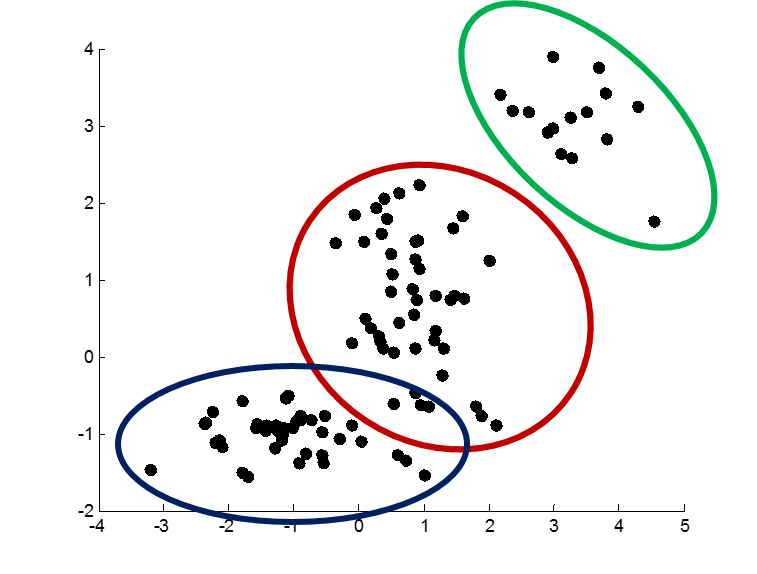
\includegraphics[scale=0.6]{fig8_2.png} 
\caption{데이터 집단 및 군집화}
\label{fig:8-2}
\end{figure} 

다음의 예시를 보자. 그림 \ref{fig:8-2}와 같이 데이터가 주어졌다면 우리는 눈대중으로 이것을 세 개의 군집으로 나눌 수 있다. 그리고 군집 내부의 점끼리는 같은 특성을 공유한다고 짐작할 수 있다. 다시 말해, 겉으로는 보이지 않는 특성을 군집화를 통해서 찾을 수 있는 것이다.  \\

\begin{figure}[ht] \centering 
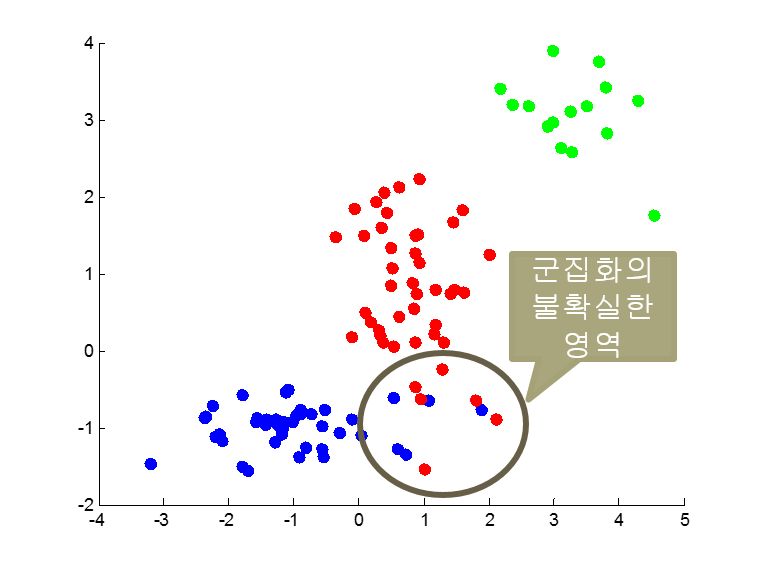
\includegraphics[scale=0.6]{fig8_1.png} 
\caption{각 데이터에 잠재해 있는 특성}
\label{fig:8-1}
\end{figure} 

한편, 데이터의 보이지 않는 특성이 그림 \ref{fig:8-1}와 같이 빨강, 파랑, 초록으로 잠재해 있다고 하자. 이것을 보았을 때 그림 \ref{fig:8-2}에서의 군집화는 잘 된 것으로 보인다. 하지만 그림 \ref{fig:8-1}에서 동그라미로 표시한 부분에서는 빨강 데이터 포인트와 파랑 데이터 포인트가 공존하고 있으며, 이를 나타내듯 그림 \ref{fig:8-2}의 군집화에서도 빨간색과 파란색 동그라미가 서로 겹친 채로 나타난다. 이 때문에, 해당 부분에 위치한 데이터가 실제로 빨강과 파랑 중에서 어떤 특성을 가지는지를 판단하기는 어렵다. 우리는 이것을 어떻게 처리하면 좋을지를 생각해야 한다. \\

\begin{figure}[ht] \centering 
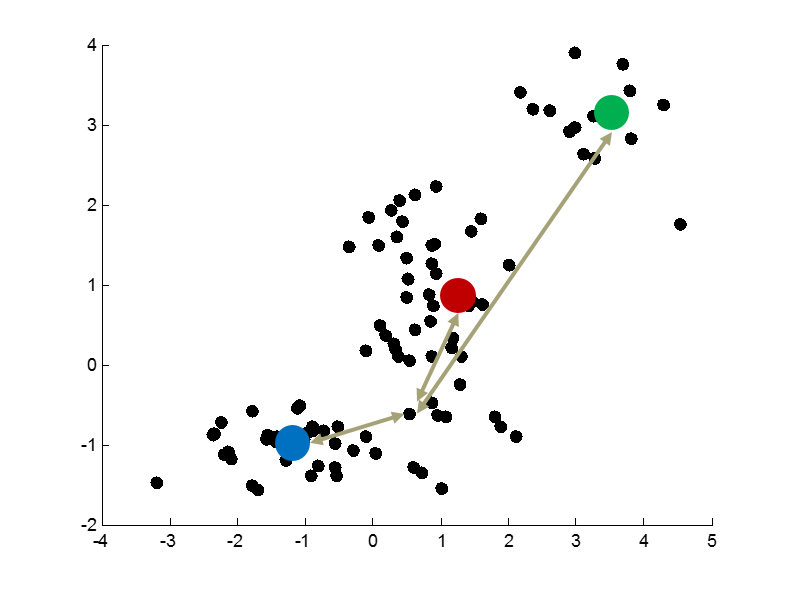
\includegraphics[scale=0.6]{fig8_4.png} 
\caption{K-평균 군집화 알고리즘}
\label{fig:8-4}
\end{figure} 

%-----------------------------------------------------------------
\subsection{K-평균 군집화}
%-----------------------------------------------------------------

%슬라이드 7
이제 K-평균 군집화 (K-Means Clustering)에 대해서 알아보겠다. K-평균 군집화는 내부적인 특성의 종류가 K개 있다고 가정하고 데이터를 가장 가까운 특성에 할당하는 알고리즘을 말한다. 단, 여기서 데이터를 나누는 기준이 되는 특성 또는 중심은 사전에 정해진 것이 아니며, 알고리즘을 반복하는 과정에서 변할 수 있다. \\

예를 들어, 우리에게는 특성이 주어지지 않은 검은색 점들이 있으며, 우리는 이것들을 최적으로 할당해야 한다. 여기서 주의해야 할 것은 군집의 개수는 K개로 정해져 있지만 개별 군집의 중심이 주어지지는 않았다는 점이다. 우리는 각 군집의 중심을 찾아야 한다. K-평균 군집화에서는 먼저 임의로 K개의 중심을 정하고 그림 \ref{fig:8-4}에서처럼 각각의 점을 가장 가까운 중심에 할당해야 한다. 그리고 그 결과로 나타나는 K개의 군집에 대해서 또다시 중심을 찾아서 각 점들을 가장 가까운 새로운 중심에 할당해야 한다. K-평균 군집화를 실행하기 위해서는 이러한 과정을 계속 반복해야 한다. 다시 말해, 개별 군집의 중심(Centroid)을 잡고, 각 점들을 가장 가까운 중심에 할당해서 새로운 군집을 구성하는 것을 계속 반복하는 것이 바로 K-평균 군집화의 과정인 것이다. \\   

\begin{figure}[ht] \centering 
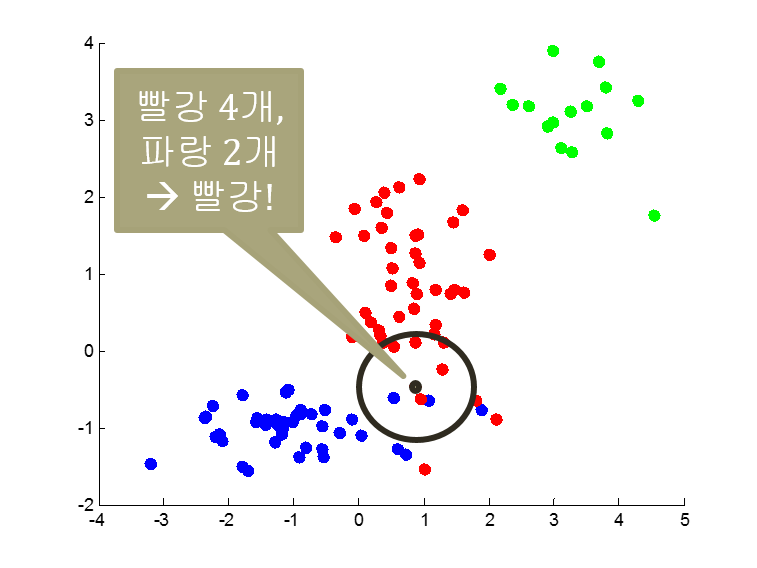
\includegraphics[scale=0.6]{fig8_3.png} 
\caption{K-최근접 이웃 알고리즘}
\label{fig:8-3}
\end{figure} 

K-평균 군집화는 얼핏 보면 K-최근접 이웃 알고리즘과 비슷해 보인다. 여기서 K-최근접 이웃 알고리즘(K-Nearest Neighbors algorithm)이란 새로운 데이터의 특성을 판정할 때, 데이터로부터 가장 가까운 K개의 기존 데이터에서 가장 많은 수의 데이터가 가진 특성을 새로운 데이터의 특성으로 정하는 알고리즘을 말한다. 그러나 이 알고리즘을 수행하기 위해서는 학습을 위한 기존 데이터의 특성이 주어져 있어야 하므로 지도 학습에 속한다. 따라서 자율 학습인 K-평균 군집화와는 구별된다. \\

이제 최적화의 관점에서 보다 자세하게 군집화 문제를 생각해 보자. 개별 군집에 속한 데이터 포인트와 군집의 무게 중심의 거리를 모두 더하면 다음의 식이 나온다. 
\begin{equation}
J = \sum_{n=1}^{N} \sum_{k=1}^{K} r_{nk} \lVert x_{n} - \mu_{k} \rVert^{2}
\label{eq:8-1}
\end{equation}
여기서 $x_{n}$은 $n$번째 데이터 포인트의 위치를 나타내는 상수값이며, $\mu_{k}$는 $k$번째 중심의 위치를 나타내는 결정 변수(Decision Variable)이다. 또한, $r_{nk}$는 $n$번째 데이터 포인트가 $k$번째 군집에 속하면 1, 속하지 않으면 0의 값을 가지는 이진 결정 변수로서 데이터의 할당 정보를 나타낸다. 이 때, 우리는 $x$가 주어졌을 때 $J$를 최소로 만드는 $\mu$와 $r$을 알아내야 한다. 단, 한 가지 주의할 점은 하나의 데이터 포인트를 반드시 하나의 군집에 할당해야 한다는 것다. 다시 말해, 모든 $n$에 대해서 $\sum_{k=1}^{K} r_{nk}=1$을 만족해야 한다. \\

어떻게 $J$를 최적화할 수 있을까? 이전 단원에서 다루었던 선형 회귀, 로지스틱 회귀에서는 결정 변수가 한 종류였기 때문에 목적 함수를 미분해서 최적의 결정 변수값을 구할 수가 있었다. 하지만 여기서는 두 종류의 결정 변수가 있는데다 그 중 하나인 $r_{nk}$는 0 또는 1의 값을 가진 이진 결정 변수이기 때문에 함부로 $r_{nk}$에 대해서 미분을 진행할 수 없다. K-평균 군집화에서는 $r$이 정해진 채로 최적의 $\mu$를 정하고, $\mu$가 정해지면 다시 최적의 $r$을 할당하는 식으로 알고리즘을 진행한다. 다시 말해서 K-평균 군집화는 중심의 위치 $\mu_{k}$와 데이터의 할당 정보 $r_{nk}$를 상호적으로(Interacting) 변화시키면서 $J$의 값을 반복적으로 줄여나가는 반복 최적화(Iterative Optimization) 알고리즘이다. \\

%슬라이드 8
K-평균 군집화의 정확한 반복 최적화 과정은 다음과 같다. 처음 군집화를 시작할 때에는 $\mu$값을 임의로 정해준다. 이후에는 다음의 과정을 반복해서 진행한다. 먼저 $\mu$가 정해져 있을 때는 각 $n$에 대해서 $n$번째 데이터 포인트로부터 가장 가까운 중심을 찾아서 그 중심이 나타내는 $k'$번째 군집에 대해서는 $r_{nk'}=1$로 정하고 그 외의 군집에 대해서는 모두 $r_{nk}=0$으로 정해준다. 그리고 $r$이 정해져 있을 때에는 수식 (\ref{eq:8-2})에서와 같이 각 군집별 무게 중심을 찾아서 $\mu$값으로 정해준다.  
\begin{equation}
\mu_{k} = \frac{\sum_{n=1}^{N} x_{n}r_{nk} }{ \sum_{n=1}^{N} r_{nk} }
\label{eq:8-2}
\end{equation}

왜 하필이면 무게 중심을 사용하는 것일까? 앞에서 말한 미분을 사용해서 이것을 보일 수 있다. $r$이 주어져 있을 때 문제의 결정 변수는 $\mu$밖에 없으며, $\mu$에는 특별한 제약이 없으므로 우리는 목표 함수 $J$를 각각의 $\mu_k$에 대해서 미분할 수 있다. 
\begin{eqnarray}
\frac{dJ}{d\mu_k} & = & \frac{d}{d\mu_k} \sum_{n=1}^{N} \sum_{k=1}^{K} r_{nk} \lVert x_{n} - \mu_{k} \rVert^{2} \nonumber \\
& = & \frac{d}{d\mu_k} \sum_{n=1}^{N} r_{nk} \lVert x_{n} - \mu_{k} \rVert^{2} \nonumber \\
& = & -2 \ \sum_{n=1}^{N} r_{nk} (x_{n} - \mu_{k}) \nonumber \\
& = & -2 \ (\sum_{n=1}^{N} r_{nk}x_{n} - (\sum_{n=1}^{N} r_{nk})\mu_{k} ) \label{eq:8-3}
\end{eqnarray}
이 때, $\mu$가 최적해라면 각 $k$에 대해서 ${dJ}/{d\mu_k}=0$를 만족해야 하므로, 최적해는 수식 (\ref{eq:8-2})와 같다. 여기서 $\mu_{k}$의 분모는 $k$번째 군집에 할당된 데이터 포인트의 개수를, 분자는 $k$번째 군집에 할당된 데이터 포인트의 좌표값 총합을 나타낸다. 따라서 이것은 $k$번째 군집에 할당된 데이터 포인트의 평균 좌표값인 무게 중심과 같다. \\

K-평균 군집화의 과정을 일반적으로 기댓값 최대화 알고리즘(Expectation-Maximization Algorithm) 또는 줄여서 EM 알고리즘(EM Algorithm)이라고 한다. EM 알고리즘에는 주어진 파라미터에 대한 로그 우도(Log-Likelihood)의 기댓값을 구하는 과정과 로그 우도를 최대화하는 파라미터를 찾는 과정이 있으며, 이들 과정을 반복해서 진행하는 것이 바로 EM 알고리즘이다. 여기서는 각 데이터 포인트를 가장 가까운 군집에 할당하는 과정을 기댓값 과정, 각 군집의 중심을 최적으로 갱신하는 과정을 최대화 과정으로 볼 수 있다. EM 알고리즘에 대해서는 뒤에서 더욱 자세히 다루겠다. \\

%슬라이드 9
\begin{figure}[ht] \centering 
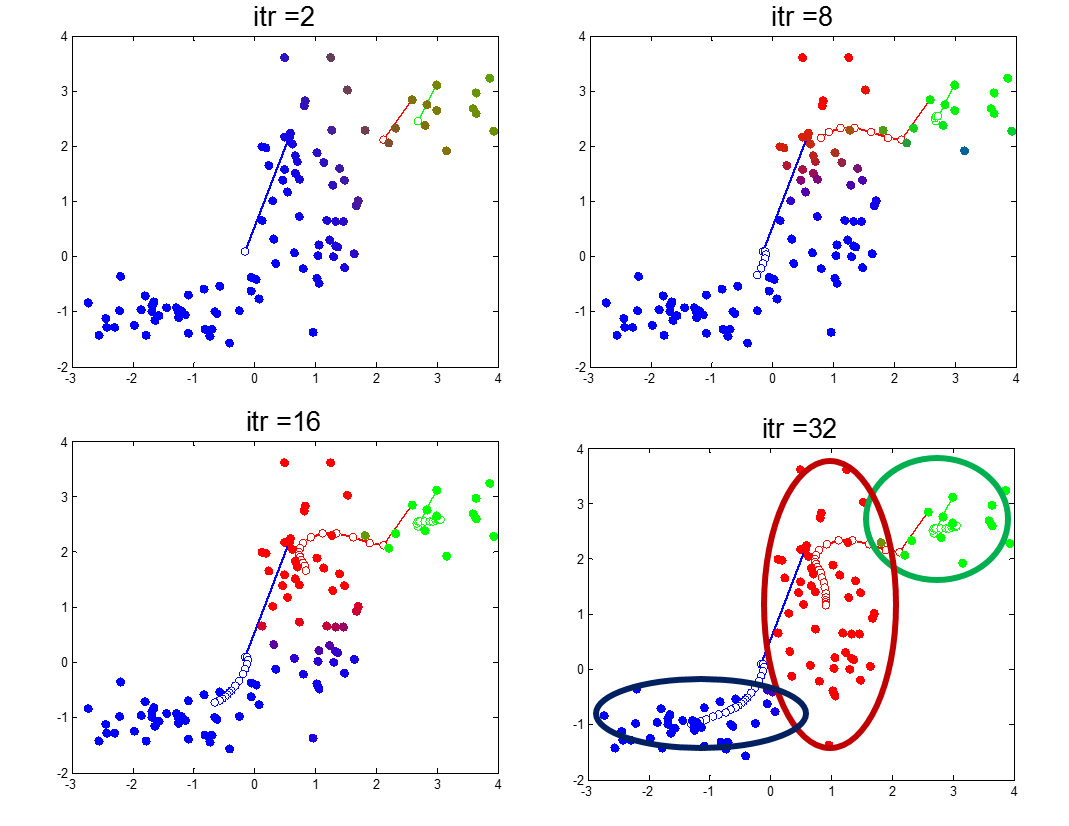
\includegraphics[scale=0.7]{fig8_6.png} 
\caption{K-평균 군집화의 실행}
\label{fig:8-6}
\end{figure} 

그림 \ref{fig:8-6}의 그래프들은 K-평균 군집화를 Matlab으로 구현한 결과이다. 검은색 점은 개별 데이터 포인트를, 흰색 점은 군집의 중심을 나타낸다. 여기서는 반복적인 군집화 과정에서 군집의 중심과 형태가 함께 변하는 것을 확인할 수 있다. \\

\begin{figure}[ht] \centering 
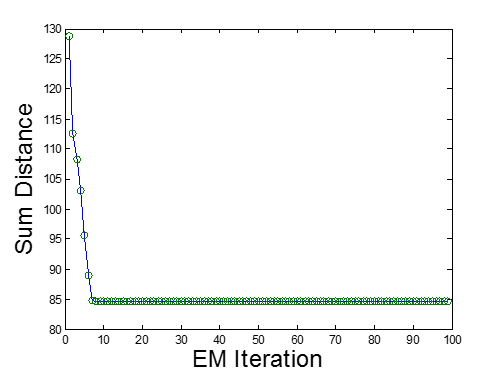
\includegraphics[scale=1.0]{fig8_5.png} 
\caption{EM 반복에 따른 목표함수의 값 변화}
\label{fig:8-5}
\end{figure} 

그림 \ref{fig:8-5}의 그래프는 K-평균 군집화의 반복 횟수에 따른 목표함수의 값 변화를 나타낸다. 이 그래프는 처음 몇 번의 반복은 목표함수의 값을 개선시키지만, 반복 횟수가 10번을 넘어가면 목표 함수의 개선이 없어 더 이상의 반복은 무의미하다는 것을 말하고 있다. 이렇게 반복 최적화 과정에서 특정 값으로 수렴한 해를 지역 최적해(Local Optimum)라고 한다. 지역 최적해 주변에서는 그것보다 더 좋은 해를 찾을 수 없으므로 K-평균 군집화는 좋은 알고리즘이라고 할 수 있다. 그러나 지역 최적해는 최적화 문제의 정확한 해답인 전역 최적해(Global Optimum)와는 다를 수도 있다. 지역 최적해와 전역 최적해의 차이에 대해서는 인터넷이나 다른 책을 참고하길 바란다. \\

%슬라이드 10
K-평균 군집화는 구현하기 간편하며, 지역 최적해를 빠르게 찾을 수 있다는 장점이 있다. 그러나 K-평균 군집화에는 몇 가지 생각해 보아야 할 문제가 있다. 먼저 군집의 개수인 K값으로 무엇이 적절한지를 생각해야 한다. 데이터에 대한 사전 정보가 없는 상황에서 처음부터 적절한 K값을   찾는 것은 쉽지 않다. 적절한 K값을 찾는 방법의 하나로 비모수 베이지안(Bayesian Nonparametric)이 있으나 여기서 다루지는 않도록 하겠다. \\

알고리즘을 처음 시작하면서 중심의 위치를 잡는 것 또한 문제이다. 여기에는 임의의 K개의 데이터 포인트를 선택해서 중심으로 두고 시작하는 것 외에도 여러 다양한 방법이 있다. 그러나 처음에 중심의 위치를 제대로 잡지 않으면 이후의 과정에서 나쁜 지역 최적해에 빠질 수 있다. 이러한 위험을 고려해서 중심의 위치를 바꿔가면서 여러 번 알고리즘을 수행한다면 더욱 안정적으로 좋은 해를 구할 수 있다.  \\

데이터 포인트와 군집의 중심 사이의 거리로 유클리드 거리(Euclidean Distance)를 적용하는 것이 부적절할 수도 있다. 각 군집이 원형으로 모여있다면 유클리드 거리가 적절할 수 있으나 그렇지 않다면 다른 거리 기준을 생각해 보아야 한다. \\  

가장 큰 문제는 하나의 데이터 포인트를 반드시 하나의 군집에 할당해야 한다는 조건인 강한 군집화(Hard Clustering)로부터 나온다. 데이터를 어떤 군집에 할당해야 할지 애매한 경우, 다시 말해서 데이터와 각 군집별 중심 사이의 거리가 비슷할 경우에는 데이터를 특정 군집에 할당하는 것이 오히려 모델의 설명력을 약하게 만든다. 이 때는 어떤 군집에 할당할지를 확률값처럼 0과 1 사이의 실수로 나타내는 약한 군집화(Soft Clustering)를 적용할 수 있다.

%-----------------------------------------------------------------
\section{가우시안 혼합 모델}
%-----------------------------------------------------------------

%-----------------------------------------------------------------
\subsection{다항 분포와 다변수 가우스 분포}
%-----------------------------------------------------------------

%슬라이드 13
가우시안 혼합 모델은 K-평균 군집화의 문제점인 유클리드 거리와 강한 군집화를 해결할 수 있는 자율학습 방법에 속한다. 이러한 가우시안 혼합 모델을 이해하기 위해서는 다항 분포와 다변수 가우스 분포에 대한 이해가 있어야 한다. \\

다항 분포(Multinomial Distribution)는 이항 분포를 일반화한 것으로, 여기서의 개별 사건이란 $K$개의 선택지 $(K \geq 2)$ 중에서 정확히 하나를 선택한 것과 같다. Section 1에서 우리는 던졌을 때 앞면 또는 뒷면이 나오는 압정의 예시로 이항 분포를 이해할 수 있었다. 이처럼 던졌을 때 1, 2, 3, 4, 5, 6 중 하나가 나오는 주사위를 다항 분포의 하나의 예시로 생각할 수 있다. 압정에는 두 가지 선택지가 있듯이 주사위에는 여섯 가지 선택지가 있다. 어떤 선택지를 골랐는지 나타내기 위해서는 선택지 개수만큼의 크기를 갖는 이진 벡터 $X$를 사용한다. 예를 들어, 주사위를 던져서 3이 나오는 사건에 대해서는 세 번째 성분만 1이고 나머지 성분은 0인 벡터 $X=(0,0,1,0,0,0)$으로 사건을 표현할 수 있다. 이 때, 여러 가지 선택지가 있더라도 선택할 수 있는 것은 정확히 하나이므로 모든 사건에 대해서 $X_k$를 모두 더하면 1이 되어야 한다. 다시 말해, $\sum_{k=1}^{K} X_k = 1$이다. \\

다항 분포에서는 어떤 방식으로 확률을 정의할 수 있을까? 다항 분포에서 개별 사건이 일어날 확률을 모두 더하면 1이 되어야 한다. 예를 들어, 주사위를 던지면 1이 나올 확률, 2가 나올 확률, $\cdots$, 6이 나올 확률을 더하면 정확히 1이 된다. 개별 확률을 $\mu_k$라고 했을 때, 이것을 수식으로 나타내면 $\sum_{k=1}^{K} \mu_k = 1$이 된다. 또한, 개별 확률은 0보다 크거나 같아야 한다. 다시 말해, 각 $k$에 대해서 $\mu_k \geq 0$이다. $\mu_k$가 정해져 있을 때 특정 사건이 일어날 조건부 확률을 다음의 수식으로 나타낼 수 있다.  
\begin{equation}
P_{X}(x|\mu) = \prod_{k=1}^{K} \mu_{k}^{x_k}
\label{eq:8-4}
\end{equation}
여기서 $x_k$들 중에서는 정확히 하나만이 1의 값을 가지고 나머지는 모두 0이기 때문에, 선택지 하나에 대한 $\mu_{k}$만 남아서 해당 선택지의 확률을 나타낸다. \\

이제 N개의 데이터를 포함하는 데이터 집합 $D$가 주어졌을 때의 조건부 확률을 생각해보자. $D$의 데이터끼리는 서로 독립이므로 다음과 같이 확률의 곱으로 표현할 수 있다. 
\begin{eqnarray}
P_{X}(x|\mu) & = & P(X_{1}=x_{1},\cdots,X_{N}=x_{N}|\mu) \nonumber \\
& = &  \prod_{n=1}^{N} P_{X_{n}}(x_{n}|\mu) \label{eq:8-5}
\end{eqnarray}
여기에 수식 (\ref{eq:8-4})를 대입하고 전개하면 다음의 수식을 얻을 수 있다. 
\begin{eqnarray}
\prod_{n=1}^{N} P_{X_{n}}(x_{n}|\mu) & = & \prod_{n=1}^{N} \prod_{k=1}^{K} \mu_{k}^{x_{nk}} \nonumber \\
& = &  \prod_{k=1}^{K} \mu_{k}^{\sum_{n=1}^{N} x_{nk}} \nonumber \\
& = &  \prod_{k=1}^{K} \mu_{k}^{m_k} \label{eq:8-6}
\end{eqnarray}
여기서 $m_k=\sum_{n=1}^{N} x_{nk}$는 $N$개의 데이터 중에서 $k$번째 선택지의 값을 가지는 데이터 포인트의 개수와 같다. 따라서 $\mu$의 최우추정값을 찾기 위해서는 $\mu_k \geq 0, \ k=1,\cdots,K$과 $\sum_{k=1}^{K} \mu_k = 1$을 만족시키면서 $P(X|\mu)=\prod_{k=1}^{K} \mu_{k}^{m_k}$을 최대화하는 $\mu$를 찾아야 한다. 그렇다면 최적의 $\mu$를 어떻게 찾을 수 있을까? \\

%슬라이드 14
우리는 앞서 chapter 5에서 사용했던 라그랑지 방법으로 최적의 $\mu$를 찾을 수 있다. 다시 한 번 설명하면, 라그랑지 방법(Lagrange Method)은 조건 함수와 제약식이 있는 최적화 문제를 풀기 위한 방법이며, 그것의 구체적인 과정은 다음과 같다. 먼저, 제약식의 우변을 0으로 만든 뒤, 좌변에 라그랑지 승수(Lagrange Multiplier)를 곱하고 이를 제약식에 더해서 라그랑지 함수(Lagrange Function)를 구성한다. 다음으로, 라그랑지 함수를 각 변수에 대해서 편미분한 뒤, 그것들이 0과 같다는 식을 세운다. 마지막으로, 이전 과정에서 나온 식을 본래의 조건식과 함께 활용해서 최적해와 최적값을 구한다. \\

이러한 과정을 다음과 같이 우리의 문제에 적용할 수 있다. 먼저, 제약식 $\sum_{k=1}^{K} \mu_k - 1 = 0$에 라그랑지 승수 $\lambda$를 곱하고 이를 제약식에 로그를 씌운 로그 우도에 더해서 라그랑지 함수를 구성한다. 
\begin{eqnarray}
L(\mu, m, \lambda) & = &  \textrm{ln} \prod_{k=1}^{K} \mu_{k}^{m_k} + \lambda (\sum_{k=1}^{K} \mu_k - 1) \nonumber \\
& = & \sum_{k=1}^{K} m_{k} \textrm{ln} \mu_{k} + \lambda (\sum_{k=1}^{K} \mu_k - 1)  \label{eq:8-7} 
\end{eqnarray}
다음으로, 수식 (\ref{eq:8-7})을 각 $\mu_k$ 에 대해서 편미분하고, 그것들이 0과 같다는 식을 세운다. 
\begin{equation}
\frac{d}{d \mu_{k}}L(\mu, m, \lambda)  =  \frac{m_k}{\mu_k} + \lambda = 0  \label{eq:8-8} 
\end{equation}
마지막으로, 수식 (\ref{eq:8-8})을 $\mu_k$에 대한 식으로 나타내면
\begin{equation}
\mu_k =  - \frac{m_k}{\lambda} \label{eq:8-9} 
\end{equation}
와 같으며, 수식 (\ref{eq:8-9})를 모든 $k$에 대해서 더하면, 
\begin{equation}
\sum_{k=1}^{K} \mu_k =  - \sum_{k=1}^{K} \frac{m_k}{\lambda} = 1 \label{eq:8-10} 
\end{equation}
이다. 이를 달리 표현하면
\begin{equation}
\lambda = - \sum_{k=1}^{K} m_k = -N \label{eq:8-11} 
\end{equation}
이 된다. 그리고 이를 수식 (\ref{eq:8-9})에 대입하면 다음과 같이 $\mu_k$의 값을 $m_k$와 $N$으로 나타낼 수 있다.  
\begin{equation}
\mu_k =  \frac{m_k}{N} \label{eq:8-12} 
\end{equation}
또한, 수식 (\ref{eq:8-12})에서의 각 $\mu_k$값은 음수가 아니므로, $\mu \geq 0$ 또한 만족한다. 따라서 수식 (\ref{eq:8-12})의 $\mu$는 수식 (\ref{eq:8-5})의 $P(X|\mu)$를 최대로 만든다. 이러한 $\mu$를 다항 분포의 최우추정량(Maximum Likelihood Estimator, MLE)이라고 한다. \\

%슬라이드 15-1
다음으로 다변수 가우스 분포에 대해서 알아보자. 다변수 가우스 분포(Multivariate Gaussian Distribution) 또는 다변수 정규분포(Multivariate Normal Distribution)는 변수가 하나인 가우스 분포를 여러 개의 변수를 가질 수 있도록 일반화한 것을 말한다. 일단, 기초 통계학을 배웠다면 기댓값(Expectation) $\mu$와 분산(Variance) $\sigma^2$을 가지는 가우스 분포의 확률 밀도 함수(Probability Density Function)가 다음과 같다는 사실을 알고 있을 것이다. 
\begin{equation}
N(x|\mu, \sigma^2) = \frac{1}{\sqrt{2 \pi \sigma^2}} \textrm{exp}(-\frac{1}{2 \sigma^2} (x-\mu)^2) \label{eq:8-13} 
\end{equation}
이 때, 일차원 변수인 $x \in \mathbb{R}$를 다차원 벡터 $ {x} \in {\mathbb{R}}^{D}$로 확장하기 위해서는 $x$가 가진 성질인 평균과 분산의 개념 또한 보다 일반화해주어야 한다. 사실, 평균에 대해서는 비교적 간단히 일반화할 수 있다. 우리가 다변수 가우스 분포에서 평균값 벡터 $ {\mu} \in {\mathbb{R}}^{D}$를 정의한다면, 각 $x_j$에 대한 평균은 $ {\mu}$의 $j$번째 성분인 $\mu_j$인 것이다. 그러나 분산을 다변수의 경우로 일반화하기 위해서는 각 $x_j$의 분산 외에도 서로 다른 $x_i$와 $x_j$의 상관관계(correlation) 또한 생각해야 한다. 그러나 이러한 개념들을 일일이 나타내는 것은 그렇게 깔끔한 표현이 아닐 것이다. \\

%슬라이드 16
다변수 분포의 경우에서 분산과 상관관계를 하나의 개념으로 나타낸 것이 바로 공분산 행렬(covariance matrix)이다. 공분산 행렬 $ {\Sigma}$에서는 주대각성분인 $ {\Sigma}_{jj}$는 $x_j$의 분산을, 그 외의 $ {\Sigma}_{ij}$는 $x_i$와 $x_j$의 상관관계를 나타낸다. 또한, 특정 행렬이 공분산 행렬이기 위해서는 반드시 정부호 행렬(Positive-Definite Matrix)이여야 한다. 이것은 행렬 $ {\Sigma}$가 모든 $i$, $j$에 대해서 $ {\Sigma}_{ij}$와 $ {\Sigma}_{ji}$의 값이 같은 대칭 행렬(Symmetric Matrix)이여야 할 뿐만 아니라, 모든 영벡터가 아닌 벡터 $ {z} \in {\mathbb{R}}^{D} \setminus \{  {0} \}$에 대해서 $ {z}^{T}  {\Sigma}  {z}$가 반드시 양수여야 한다는 것을 말한다. \\

\begin{figure}[ht] \centering 
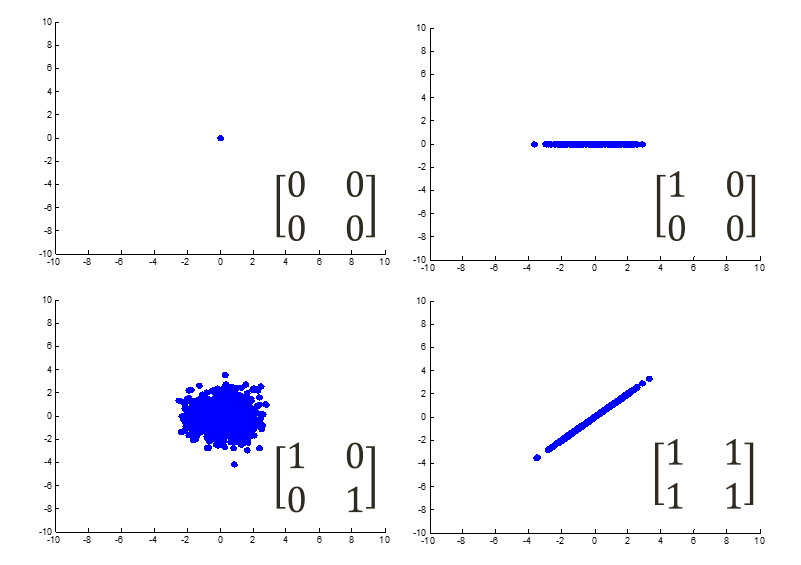
\includegraphics[scale=0.6]{fig8_7.png} 
\caption{공분산 행렬에 따른 다변수 가우스 분포 1}
\label{fig:8-7}
\end{figure} 

공분산 행렬을 쉽게 이해하기 위해서 그림 \ref{fig:8-7}에서 변수가 두 개인 다변수 가우스 분포의 몇 가지 예시를 살펴보겠다. 공분산 행렬의 모든 성분이 0이라면 $x_1$과 $x_2$ 둘 다 분산이 0이므로 값은 상수가 된다. 따라서 그러한 다변수 가우스 분포의 그래프에는 점 하나만이 나타난다. 공분산 행렬의 1행 1열 성분만이 1이고 나머지는 모두 0이라면 $x_1$의 분산은 1이므로 $x_1$만 놓고 보면 이것은 일변수 가우스 분포이며, $x_2$의 분산은 0이므로 $x_2$는 일정한 값을 가진다. 또한, $x_1$과 $x_2$ 사이에는 상관관계가 없으므로 이들 변수 사이에는 어떠한 관련도 없다. 따라서 이것들을 결합한 다변수 가우스 분포의 그래프는 $x_1$-축에 평행한 선의 형태로 나타난다. 공분산 행렬이 단위행렬(Identity Matrix)이라면 $x_1$과 $x_2$ 모두 분산이 1이고 이들 사이에는 상관관계가 없으므로 분포 그래프의 형태는 원형으로 나타난다. 공분산 행렬의 모든 성분이 1이라면 $x_1$과 $x_2$ 사이에는 1이라는 매우 강력한 상관관계가 있으므로, $x_1$과 $x_2$는 완전한 정비례 관계이다. 따라서 이것의 분포 그래프에서는 기울기가 일정한 선형 관계를 확인할 수 있다. \\

\begin{figure}[ht] \centering 
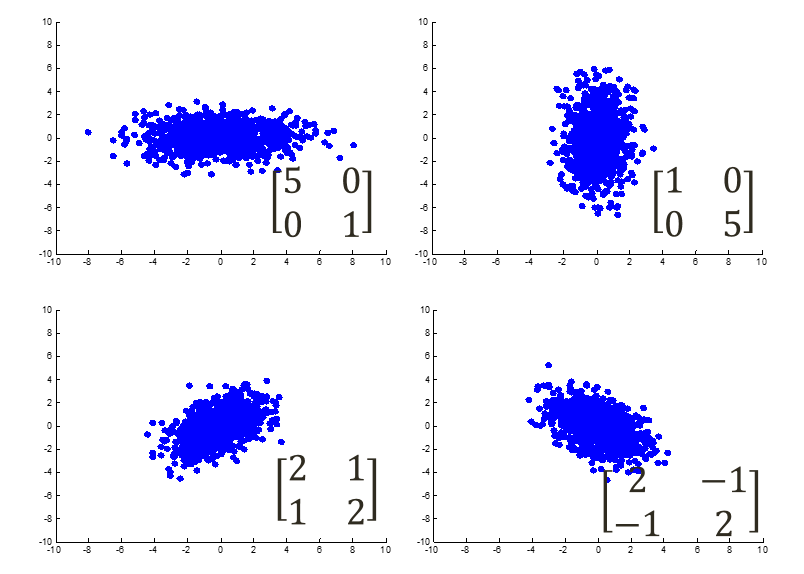
\includegraphics[scale=0.6]{fig8_8.png} 
\caption{공분산 행렬에 따른 다변수 가우스 분포 2}
\label{fig:8-8}
\end{figure} 

조금 더 복잡한 형태의 예시를 그림 \ref{fig:8-8}에서 확인할 수 있다. 먼저, $x_1$과 $x_2$의 분산이 서로 다르지만 상관관계는 없는 경우에 분포 그래프는 한 쪽이 길고 다른 쪽 축은 짧은 타원형으로 나타난다. 또한, 같은 분산 값을 가지더라도 상관관계가 있다면 마찬가지로 타원형 분포 그래프를 관찰할 수 있으며, 상관관계가 음수일 경우에도 이는 마찬가지이다. 공분산 행렬을 잘 사용하면 다양한 다변수 가우스 분포의 형태를 표현할 수 있다. 따라서 이것은 원 모양의 군집 외에 다른 형태의 군집을 제대로 설명할 수 있었던 k-평균 군집화의 문제점을 극복할 수 있는 좋은 수단이 된다. \\

%슬라이드 15-2
이제 다변수 가우스 분포의 평균값 벡터인 $ {\mu}$ 외에 공분산 행렬인 ${\Sigma}$를 정의하고 설명했으니 이것의 확률 밀도 함수를 다음과 같이 나타낼 수 있다. 
\begin{equation}
N( {x}| {\mu},  {\Sigma}) = \frac{1}{(2 \pi)^{D/2}} \frac{1}{| {\Sigma}|^{1/2}} \textrm{exp}(-\frac{1}{2} ( {x}- {\mu})^{T}  {\Sigma}^{-1} ( {x}- {\mu})) \label{eq:8-14} 
\end{equation}
여기서 $D$는 다변수 가우스 분포의 성분 갯수를, $| {\Sigma}|$는 $ {\Sigma}$의 행렬식(Determinant) 값을 의미한다. 이제 최우추정값을 구하기 위해서 다음과 같이 로그 우도를 구성할 수 있다. 
\begin{equation}
\textrm{ln} N( {x}| {\mu},  {\Sigma}) = -\frac{1}{2} \textrm{ln}| {\Sigma}| -\frac{1}{2} ( {x}- {\mu})^{T}  {\Sigma}^{-1} ( {x}- {\mu}) +  {C} \label{eq:8-15} 
\end{equation}
여기서 $ {C}$는 상수인 $(2 \pi)^{-D/2}$를 뜻하며, 최우추정량을 구하는 데 있어 영향을 주지 못하므로 무시해도 좋은 항이다. 그리고 다변수 가우스 분포의 확률값이 $ {x}_1,\cdots, {x}_N$가 주어진다면, 서로 다른 $ {x}_n$끼리는 독립이므로 로그 우도는 다음과 같이 나타난다. 
\begin{equation}
\textrm{ln} N( {X}| {\mu},  {\Sigma}) = -\frac{N}{2} \textrm{ln}| {\Sigma}| - \frac{1}{2} \sum_{n=1}^{N} ( {x}_n- {\mu})^{T}  {\Sigma}^{-1} ( {x}_n- {\mu}) \label{eq:8-16} 
\end{equation}
여기에서 수식 (\ref{eq:8-16})을 $ {\mu}$에 대해서 편미분하면, 
\begin{equation}
\frac{d}{d {\mu}} \textrm{ln} N( {X}| {\mu},  {\Sigma}) =  {\Sigma}^{-1} \sum_{n=1}^{N} ( {x}_n- {\mu}) = 0 \label{eq:8-17} 
\end{equation}
이 되므로 $ {\mu}$의 최우추정량은 다음과 같이 나타난다.
\begin{equation}
\hat{ {\mu}} = \frac{1}{N} \sum_{n=1}^{N}  {x}_{n} \label{eq:8-18} 
\end{equation}
마지막으로 수식 (\ref{eq:8-16})을 다음을 활용해서 ${\Sigma}^{-1}$에 관한 식으로 표현할 수 있으며,
\begin{equation}
\textrm{ln}|{\Sigma}| = \textrm{ln}(1/|{\Sigma}^{-1}|) = -\textrm{ln}|{\Sigma}^{-1}| \label{eq:8-18-1} 
\end{equation}
이것을 다음의 행렬식에 관한 미분 공식을 활용해서,
\begin{equation}
\frac{d}{dA} \textrm{ln}|A| = (A^{-1})^{T} \label{eq:8-18-2} 
\end{equation}
${\Sigma}^{-1}$에 대해서 편미분하면, 
\begin{equation}
\frac{d}{d {\Sigma}^{-1}} \textrm{ln} N( {X}| {\mu},  {\Sigma}) = \frac{N}{2}  {\Sigma} - \frac{1}{2} \sum_{n=1}^{N} ( {x}_n- {\mu})  ( {x}_n- {\mu})^{T} = 0 \label{eq:8-19} 
\end{equation}
이 되므로 ${\Sigma}$의 최우추정량은 다음과 같이 나타난다.
\begin{equation}
\hat{ {\Sigma}} = \frac{1}{N} \sum_{n=1}^{N} ( {x}_n-\hat{ {\mu}})  ( {x}_n-\hat{ {\mu}})^{T} \label{eq:8-20} 
\end{equation}
사실, 여기서는 구체적인 계산 과정을 생략했지만 $D$가 2와 같은 작은 값에서 수식 (\ref{eq:8-20})이 참임을 확인하는 것은 그렇게 어렵지 않을 것이다. \\

%-----------------------------------------------------------------
\subsection{가우시안 혼합 모델}
%-----------------------------------------------------------------
%슬라이드 16
앞에서 설명한 다항 분포와 다변수 가우스 분포를 활용해서 이제는 K-평균 군집화와 같은 자율 학습의 방법인 가우시안 혼합 모델을 설명할 수 있다. 그러나 그 전에 보다 일반적인 개념인 혼합 모델에 대해서 설명하고자 한다. \\

\begin{figure}[ht] \centering 
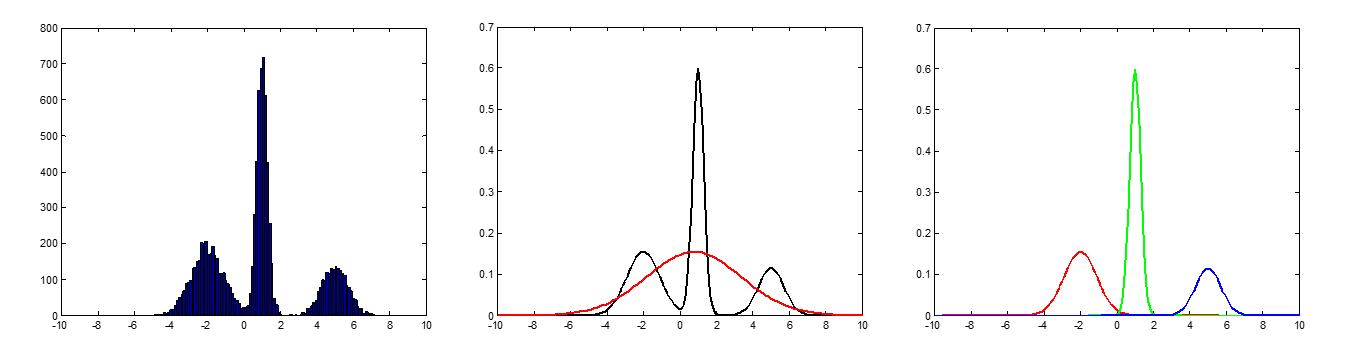
\includegraphics[scale=0.5]{fig8_9.png} 
\caption{혼합 모델에 따른 분류}
\label{fig:8-9}
\end{figure} 

그림 \ref{fig:8-9}의 첫 번째 그림에서처럼 데이터를 관찰한 결과로 히스토그램이 주어졌다고 하겠다. 이것을 정규 분포로 가정한다면 주어진 데이터의 평균과 표준편차를 구해서 두 번째 그림의 빨간색 그래프처럼 나타낼 수 있겠으나, 주어진 데이터와는 형태가 많이 다르게 된다. 한편, 첫 번째 그림의 히스토그램을 관찰하면 여기에 세 개의 봉우리가 나타나는 것을 확인할 수 있으며, 우리는 이들이 근본적으로 다르다는 가정을 할 수 있다. 이렇게 근원이 다른 여러 개의 데이터가 섞여서 하나의 데이터 집합으로 나타나는 경우에 대해서 이전까지처럼 하나의 모집단(Population)을 가정하고 모델을 세운다면 현실을 제대로 설명할 수 없게 된다. 그 때문에, 예시에서처럼 모집단이 여러 개의 부분 모집단(Subpopulation)이 결합해서 생긴 것으로 보일 때에는 여러 개의 확률 분포를 섞어서 하나의 확률 분포로 만든 혼합 모델(Mixture Model)을 적용해야 한다. 한편, 앞에서의 예시에 혼합 모델을 적용한다면 그림 \ref{fig:8-9}의 세 번째 그림에서처럼 빨간색, 녹색, 파란색의 세 가지 부분 모집단으로 표현할 수 있다. \\

혼합 모델을 정확히 이해하기 위해서 수식 표현을 빌리도록 하겠다. 확률 변수 $X$가 평균이 $\mu_k$이고, 분산이 $\sigma_{k}^{2}$인 여러 개의 정규 분포를 따르는 확률 변수 $X_{1},\cdots,X_{K}$의 혼합이라면 이것의 분포 함수는 다음과 같이 나타난다. 
\begin{equation}
P_{X}(x) = \sum_{k=1}^{K} \pi_{k} N(x|\mu_k,\sigma_{k}) \label{eq:8-21} 
\end{equation}
$N(x|\mu,\sigma)$는 정규 분포의 확률 밀도 함수이며, $\pi_{k}$는 개별 확률 변수에 대한 혼합 계수(Mixing Coefficients)이다. 혼합 계수는 $X$ 전체에서 $X_{k}$가 얼마나 자주 나타나는지를 확률적으로 표현한다. 그 때문에 각 $k$에 대해서 $\pi_{k}$는 0보다 크거나 같아야 하며, 모든 $\pi_{k}$를 합한 것은 정확히 1이 되어야 한다. 이것을 보다 일반화해서 확률 변수 $Z$로 표현하고, 여기에 더해 각각의 $X_{k}$를 일반적인 확률 변수로 생각한다면 $X$의 분포 또한 다음과 같이 보다 일반적인 형태로 나타낼 수 있다. 
\begin{equation}
P_{X}(x) = \sum_{k=1}^{K} P_{Z}(z^k) P_{X}(x|Z=z^k) \label{eq:8-22} 
\end{equation}
여기서 $z^k$는 $k$번째 성분이 1이고 나머지는 모두 0인 벡터이며, $P_{Z}(z^k)$는 $Z$가 $z^k$와 같을 확률을 나타내는 분포 함수이다. 따라서 이것은 $X$ 전체에서 $X_{k}$가 나타날 확률을 나타내기도 한다. $P_{X}(x|Z=z^k)$는 $X_{k}$로부터 나온 부분 모집단의 확률 밀도 함수로서 이것을 따로 혼합 구성 요소(Mixture Component)라고 한다. 

%슬라이드 17-1
가우시안 혼합 모델은 $Z$가 다항 분포, 각각의 $X_{k}$가 다변수 가우스 분포를 따르는 확률 변수인 혼합 모델의 특수한 경우이다. 따라서 $Z$의 분포 함수 $P_{Z}(z)$는 다항 분포의 분포 함수를 그대로 따온 것과 같다. 
\begin{equation}
P_{Z}(z) = \prod_{k=1}^{K} \pi_{k}^{z_k} \label{eq:8-23} 
\end{equation}
여기서의 $z$의 각 성분 $z_k$는 0 또는 1의 값을 가지며, 이것들을 모두 합하면 1이 된다. 또한 특정 $z_k$가 1이 되고 나머지가 모두 0이 될 확률은 앞에서 설명한 혼합 계수인 $\pi_{k}$이다. 한편, 혼합 구성 요소이면서 $X_k$의 확률 밀도 함수와 같은 $P_{X}(x|Z=z^{k})$는 다변수 가우스 분포의 확률 밀도 함수에 따라서 다음과 같은 형태로 나타난다. 
\begin{equation}
P_{X}(x|Z=z) = N(x|{\mu}_{k}, {\Sigma}_{k}) = \prod_{k=1}^{K} N(x|{\mu}_{k}, {\Sigma}_{k})^{z_{k}} \label{eq:8-24} 
\end{equation}
군집화의 관점에서 이것은 하나의 데이터 포인트가 개별 군집에 있을 확률이 각각 있고, 군집별로 그것의 원천으로 생각되어지는 다변수 가우스 분포가 있다는 것이 된다. \\

\begin{figure}[ht] \centering 
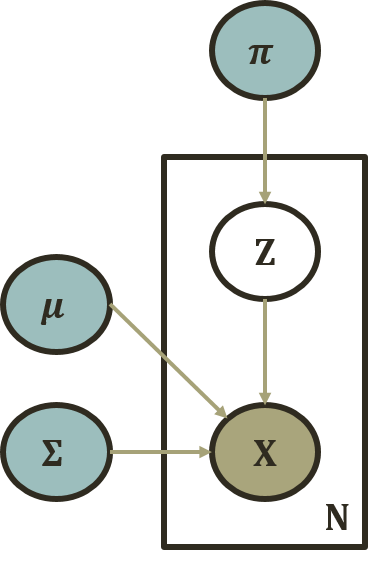
\includegraphics[scale=0.6]{fig8_10.png} 
\caption{가우시안 혼합 모델의 베이지안 네트워크}
\label{fig:8-10}
\end{figure} 

한편, 가우시안 혼합 모델을 그림 \ref{fig:8-10}에서와 같이 베이지안 모델로 나타낼 수 있다. 이 베이지안 네트워크에서 ${\mu}$와 ${\Sigma}$는 다변수 가우스 분포의 평균값 벡터와 공분산 행렬을, $\pi$는 다항 분포에서의 개별 확률값을 나타내며, 이것들이 확률 변수의 파라미터라는 것을 표현하기 위해서 특별히 파란색으로 칠하였다. 확률 변수로는 $Z$와 $X$가 있으며, 이들 중 $Z$는 숨겨진 개별 데이터가 어느 군집에 속하는지를 나타내므로 색칠하지 않았지만 $X$는 관찰로 확인한 데이터 그 자체이므로 색칠해 주어야 한다. 한편, 여기에는 판 표기법이 쓰였으며 서로 독립인 $N$개의 데이터가 있다는 것을 나타낸다. 판 내부에는 $Z$와 $X$가 같이 들어 있기 때문에 각각의 $n$번째 데이터는 각각 고유한 값인 $z_n$과 $x_n$을 가지고 있으며, $x_n$은 드러나 있지만 $z_n$은 겉으로 드러나지 않는다는 것을 알 수 있다. \\ 

%슬라이드 17-3, 18
그렇다면 이제는 지금까지 관측한 데이터를 가장 잘 설명할 수 있는 파라미터 $\pi$, $\mu$, $\Sigma$를 찾으면서 각각의 데이터 포인트를 최적인 군집에 할당해 주어야 한다. 그러나 우도를 최대화해주는 $z_1,\cdots,z_N$과 $\pi$, $\mu$, $\Sigma$를 동시에 찾기는 매우 어렵다. 때문에 k-평균 군집화에서처럼 EM 알고리즘을 적용해서 문제를 해결해나가도록 하겠다. \\

먼저 파라미터 $\pi$, ${\mu}$, ${\Sigma}$가 주어졌고 각각의 데이터에 대해서 $x_n$이 나와 있을 때, $z_n$에 대한 정보를 어떻게 유추할지를 먼저 생각해보자. 이전의 k-평균 군집화에서는 $\gamma(z_{nk})$값을 도입해서 $n$번째 데이터가 $k$번째 군집에 속해 있을 때 $\gamma(z_{nk})$를 1로, 그렇지 않았을 때는 $\gamma(z_{nk})$를 0으로 정하였다. 그러나 이러한 할당은 강한 군집화에 속하며 할당의 유연성을 떨어트리면서 모델의 설명력을 약화시킨다는 문제가 있다. 따라서 이번에는 보다 유연한 할당을 위해서 강한 군집화 대신 약한 군집화를 적용하도록 하겠다. 약한 군집화에서는 $\gamma(z_{nk})$를 $n$번째 데이터가 $k$번째 군집에 속해 있을 확률값으로 생각하면서 이것을 0과 1 사이의 값으로 정하였다. 그러면 베이즈 정리(Bayes' Theorem)를 활용해서 다음과 같이 $\gamma(z_{nk})$ 값을 파라미터인 $\pi$, ${\mu}$, ${\Sigma}$와 관측한 데이터 포인트인 $x_n$에 관한 식으로 나타낼 수 있다.  
\begin{eqnarray}
\gamma(z_{nk}) & = & P_{Z}(z^{k}|x_{n}) \nonumber \\ 
& = & \frac{ P_{Z}(z^{k})P_{X}(x_{n}|Z=z^{k}) }{ \sum_{j=1}^{K} P_{Z}(z^{j})P_{X}(x_{n}|Z=z^{j}) } \nonumber \\ 
& = & \frac{ \pi_{k} P_{X}(x_{n}|Z=z^{k}) }{ \sum_{j=1}^{K} \pi_{j} P_{X}(x_{n}|Z=z^{j}) } \nonumber \\ 
& = & \frac{ \pi_{k} N(x_{n}|{\mu}_{k}, {\Sigma}_{k}) }{ \sum_{j=1}^{K} \pi_{j} N(x_{n}|{\mu}_{j}, {\Sigma}_{j}) } \label{eq:8-25} 
\end{eqnarray} 
이런 식으로 $\pi$, ${\mu}$, ${\Sigma}$, 그리고 $x_1,\cdots,x_N$이 주어진 상황에서 적절한 $\gamma$값을 찾는 과정이 바로 EM 알고리즘의 기댓값 과정이다. k-평균 군집화에서 기댓값 과정은 가장 가까운 군집에 할당하는 과정으로 $\gamma(z_{nk})$는 0 또는 1의 값만을 가졌으나, 여기서는 확률적인 의미를 지닌 0과 1 사이의 값을 가진다. \\  

%슬라이드 17-2, 19
다음은 EM 알고리즘의 최대화 과정에 대해서 생각해보자. 각각의 데이터 $x_n$에 대해서 어떤 군집에 할당될지에 대한 확률적인 정보가 미리 주어져 있을 때, 다시 말해 $\gamma$가 주어졌을때, 가장 적절한 $\pi$, ${\mu}$, ${\Sigma}$를 찾는 것이 최대화 과정이 되겠다. 이를 위해서 우리는 우도를 정의하고 최우추정값을 찾을 필요가 있다. 여기서는 다항 분포나 다변수 가우스 분포에서 최우추정값을 찾을 때처럼, 계산을 간편하게 하기 위해서 다음과 같이 로그 우도를 사용하겠다. 
\begin{eqnarray}
L(\pi, \mu, \Sigma) & = & \textrm{ln} P(X=x|\pi, \mu, \Sigma)  \nonumber \\ 
& = & \textrm{ln} \prod_{n=1}^{N} P(X_n=x_n|\pi, \mu, \Sigma)  \nonumber \\ 
& = & \sum_{n=1}^{N} \textrm{ln} P(X_n=x_n|\pi, \mu, \Sigma)  \nonumber \\ 
& = & \sum_{n=1}^{N} \textrm{ln}( \sum_{k=1}^{K}\pi_{k} N(x_{n}|{\mu}_{k}, {\Sigma}_{k})) \label{eq:8-26} 
\end{eqnarray} 

이제 $L(\pi, \mu, \Sigma)$을 각각의 $\pi$, ${\mu}$, ${\Sigma}$에 대해서 편미분해서 $L(\pi, \mu, \Sigma)$을 최대화하는 최우추정값을 찾아야 한다. 여기서 $\mu$나 $\Sigma$에 대한 제약 조건은 없기 때문에 그대로 편미분을 진행할 수 있다. 먼저 $L(\pi, \mu, \Sigma)$을 $\mu_{k}$에 대해서 편미분한 식은 다음과 같으며, 0과 같아야 한다. 
\begin{equation}
\frac{d}{d\mu_{k}} L(\pi, \mu, \Sigma) =  \sum_{n=1}^{N} \frac{ \pi_{k} N(x_{n}|{\mu}_{k}, {\Sigma}_{k}) }{ \sum_{j=1}^{K} \pi_{j} N(x_{n}|{\mu}_{j}, {\Sigma}_{j}) } \Sigma_{k}^{-1} (x_n - \mu_{k}) = 0 \label{eq:8-27} 
\end{equation}
이것을 이미 정해진 값인 $\gamma(z_{nk})$를 넣어서 정리하면 다음과 같이 나오며,  
\begin{equation}
\sum_{n=1}^{N} \gamma(z_{nk})(x_{n} - \mu_{k}) = 0 \label{eq:8-28} 
\end{equation}
수식 (\ref{eq:8-28})을 다시 정리하면 ${\mu}_{k}$에 관한 수식으로 나타낼 수 있어 이것을 최우추정값으로 삼을 수가 있다. 
\begin{equation}
\hat{\mu}_{k} = \frac{\sum_{n=1}^{N} \gamma(z_{nk}) x_n}{\sum_{n=1}^{N} \gamma(z_{nk})} \label{eq:8-29} 
\end{equation}
한편, $\Sigma_{k}$에 대해서도 마찬가지로 편미분을 적용하면,  
\begin{equation}
\frac{d}{d\Sigma_{k}^{-1}} L(\pi, \mu, \Sigma) = \sum_{n=1}^{N} (\gamma(z_{nk}) {\Sigma_{k}} - \gamma(z_{nk}) ( {x}_n- {\mu_{k}})  ( {x}_n- {\mu_{k}})^{T}) = 0 \label{eq:8-30} 
\end{equation}
와 같이 나오므로(구체적인 과정은 다변수 가우스 분포에서 $\Sigma_{k}$의 최우추정값을 구했던 과정과 동일하다),  이것을 정리해서 ${\Sigma}_{k}$에 관한 수식으로 나타내어 이것을 최우추정값이라고 정할 수 있다. 
\begin{equation}
\hat{\Sigma}_{k} = \frac{\sum_{n=1}^{N} \gamma(z_{nk}) ( {x}_n-\hat{{\mu}}_{k})  ( {x}_n-\hat{ {\mu}}_{k})^{T} }{\sum_{n=1}^{N} \gamma(z_{nk})}   \label{eq:8-31} 
\end{equation}
$\pi$에 대해서는 각각의 $\pi_k$가 음수가 아니며, $\pi_k$의 합이 1이라는 제약 조건이 있기 때문에 $\pi_k$에 대해서 편미분을 할 때에는 라그랑지 방법을 적용해야 한다. 따라서 제약식 $\sum_{k=1}^{K} \pi_{k} - 1 = 0$의 좌변에 라그랑지 상수 $\lambda$를 곱해서 우도에 더한 함수를 편미분해야 하며, 그 과정은 다음과 같다.
\begin{eqnarray}
\frac{d}{d\pi_{k}} L(\pi, \mu, \Sigma) + \lambda(\sum_{k=1}^{K} \pi_{k} - 1) & = &  \sum_{n=1}^{N} \frac{N(x_{n}|{\mu}_{k}, {\Sigma}_{k}) }{ \sum_{j=1}^{K} \pi_{j} N(x_{n}|{\mu}_{j}, {\Sigma}_{j}) } + \lambda    \nonumber  \\
& = & \frac{1}{{\pi}_{k}} \sum_{n=1}^{N} \gamma(z_{nk}) + \lambda  = 0 \label{eq:8-33} 
\end{eqnarray}
여기서 수식 (\ref{eq:8-33})의 양 변에 $\pi_{k}$를 곱해고 모든 $k$에 대해서 더한 수식은 다음과 같으며,
\begin{eqnarray}
\sum_{k=1}^{K} (\sum_{n=1}^{N} \frac{ \pi_{k} N(x_{n}|{\mu}_{k}, {\Sigma}_{k}) }{ \sum_{j=1}^{K} \pi_{j} N(x_{n}|{\mu}_{j}, {\Sigma}_{j}) } + \pi_{k} \lambda) & = & \sum_{k=1}^{K} \sum_{n=1}^{N}  \gamma(z_{nk}) + \lambda \sum_{k=1}^{K} \pi_{k}    \nonumber  \\
& = & N + \lambda = 0 \label{eq:8-34} 
\end{eqnarray}
따라서 라그랑지 상수 $\lambda$는 $-1/N$과 같다. 이제 이것을 수식 (\ref{eq:8-33})에 대입해서 ${\pi}_{k}$에 대한 식으로 정리하면 다음과 같다. 
\begin{equation}
\hat{\pi}_{k} = \frac{\sum_{n=1}^{N} \gamma(z_{nk})}{N} \label{eq:8-36} 
\end{equation}
이러한 일련의 과정을 통해서 $\pi$, ${\mu}$, ${\Sigma}$의 최우추정값을 구할 수가 있다. \\ 

가우시안 혼합 모델에서 EM 알고리즘의 최대화 과정은 $x$와 $\gamma$가 정해져 있을 때, 가장 적절한 $\pi$, ${\mu}$, ${\Sigma}$을 구하는 과정이며, 위에서 구한 최우추정값 식을 통해서 원하는 값들을 계산할 수 있다. 결국 우리는 지금까지의 과정으로 가우시안 혼합 모델에서의 기댓값 과정과 최대화 과정을 설명하였으며, 두 과정을 반복적으로 실행하면서 적절한 군집의 배치를 찾는 EM 알고리즘의 과정을 알아보았다. 다만, 맨 처음에 기댓값 과정을 시작할 때에는 $\pi$, ${\mu}$, ${\Sigma}$에 대한 정보가 없으므로 임의의 값을 정하고 나서 알고리즘을 실행해 주어야 한다. 

%슬라이드 20
\begin{figure}[ht] \centering 
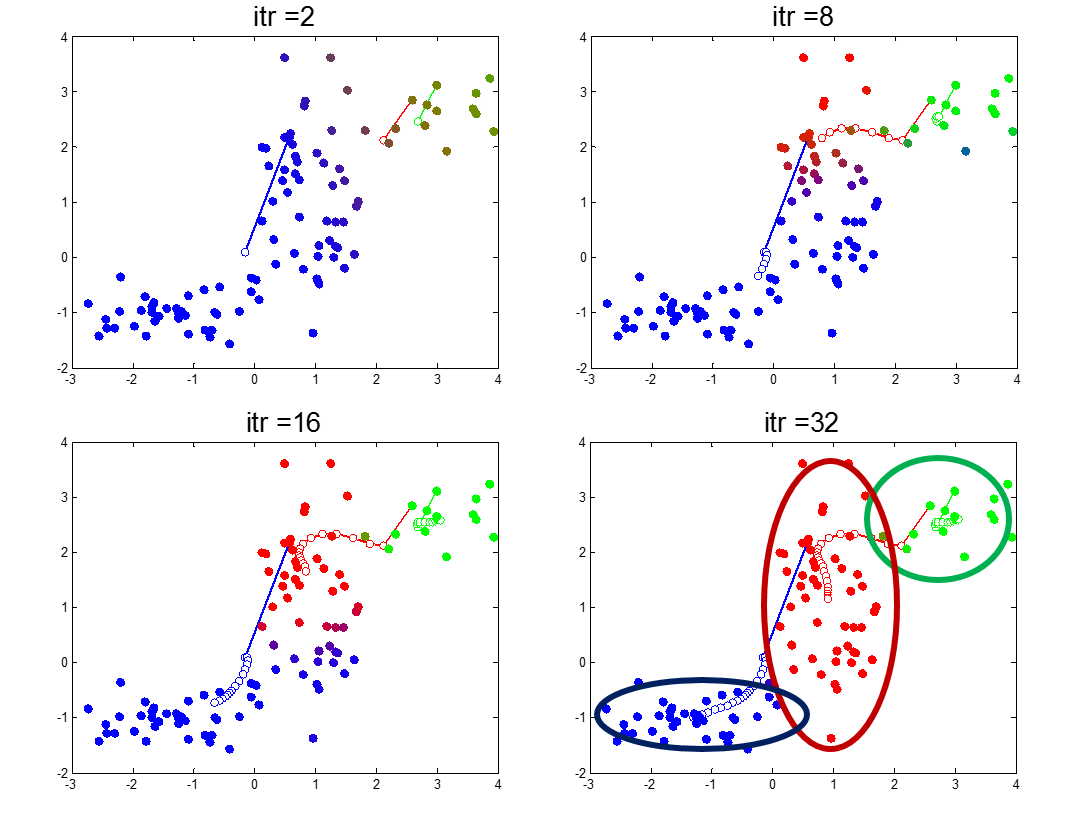
\includegraphics[scale=0.7]{fig8_11.png} 
\caption{가우시안 혼합 모델의 실행}
\label{fig:8-11}
\end{figure} 

이제는 가우시안 혼합 모델을 적용해서 EM 알고리즘의 반복으로 군집화를 시행한 결과를 확인해보자. 그림 \ref{fig:8-11}에서 반복 횟수에 따른 군집화 결과를 그래프로 확인할 수 있다. 특정 색으로 칠해진 점은 개별 데이터 포인트를, 흰색 점은 군집의 중심을 의미한다. 그러나 k-평균 군집화에서는 달리 여기서는 군집의 중심은 군집에 속한 데이터 포인트의 무게 중심이 아니라 다변수 가우스 분포의 평균값 벡터 $\mu_k$를 의미한다. 또한, $\mu_k$ 외에 공분산 행렬 $\Sigma_k$가 있기 때문에 군집의 형태가 기존 k-평균 군집화의 원형 군집에서 더 나아가 타원형 군집까지 가능하다. \\

또한, 그림 \ref{fig:8-11}에서 반복 횟수가 2회 또는 8회일 때의 그래프를 살펴보면, k-평균 군집화에서와는 다르게 빨강, 파랑, 초록 중에서 정확히 하나의 색으로만 칠해지지 않은 데이터 포인트를 관찰할 수 있다. 이것은 데이터 포인트를 특정 군집에 정확히 할당하는 대신에 군집별로 그것이 할당될 확률인 $\gamma(z_{nk})$를 설정한 것과 관련이 있다. 특정 군집에 할당될 가능성이 매우 높아 $\gamma(z_{nk})$가 1에 가까운 데이터 포인트의 경우에는 특정 군집의 색으로 확실히 칠해졌지만, $\gamma(z_{nk})$가 골고루 분산되어 있다면 데이터 포인트는 여러 개의 색이 동시에 칠해지게 된다. 이렇게 어느 군집에 들어가야 할지 애매한 데이터 포인트에 대해서 확률적인 처리를 함으로써 보다 정확히 군집화를 할 수 있다. \\

\begin{figure}[ht] \centering 
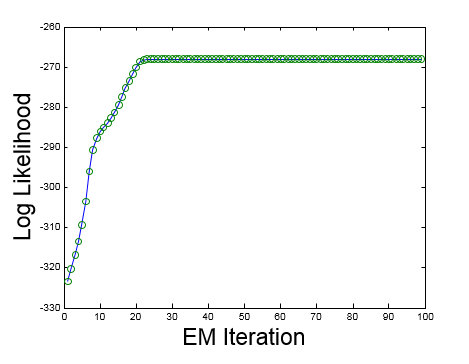
\includegraphics[scale=1.0]{fig8_12.png} 
\caption{EM 반복에 따른 목표함수의 값 변화}
\label{fig:8-12}
\end{figure} 

그림 \ref{fig:8-12}의 그래프는 EM 알고리즘의 반복 과정에서 우도값의 개선을 표현하고 있다. 그래프에 따르면 반복 횟수가 30번을 넘어가게 되면 특정 군집화의 결과로 최적해가 수렴하게 된다. 다시 말해서 파라미터 $\pi$, ${\mu}$, ${\Sigma}$와 확률 $\gamma(z_{nk})$가 특정 값으로 수렴하는 것이다. 그러나 k-평균 알고리즘과 마찬가지로 지역 최적해에 빠질 위험이 있기 때문에 나름대로 주의를 기울일 필요가 있다. \\  

%슬라이드 21
이제 가우시안 혼합 모델의 장단점에 대해서 알아보겠다. 장점으로는 무엇보다도 군집화 과정에서 더 많은 정보를 얻을 수 있다는 것이다. 가우시안 혼합 모델을 사용하면 약한 군집화로 데이터 포인트가 단순히 하나의 군집에 할당되는 것을 막기 때문에 그만큼 정보 손실을 줄일 수 있다. 또한, 잠재적인(Latent) 분포의 이해에 있어서 k-평균 군집화에서는 오로지 개별 군집의 중심만을 알 수 있었지만, 가우시안 혼합 모델을 적용한 군집화에서는 개별 군집의 중심 외에도 분포의 형태에 대한 정보를 얻을 수 있다. \\

그러나 가우시안 혼합 모델을 사용한 군집화에는 단점 또한 있다. 먼저, 가우시안 혼합 모델에는 구해야 하는 파라미터와 확률값이 많기 때문에 계산이 비교적 오래 걸린다는 단점이 있다. 또한, k-평균 군집화에서처럼 가우시안 혼합 모델을 적용한 군집화에서도 EM 알고리즘 과정에서 지역해에 빠지는 문제나, 군집의 개수인 K값을 결정하는 문제가 여전히 남아 있다. \\

%슬라이드 22
k-평균 군집화와 가우시안 혼합 모델의 차이를 수식을 통해서 좀 더 구체적으로 알아보겠다. 먼저 다변수 가우스 분포의 확률 밀도 함수를 수식 (\ref{eq:8-14})에서 빌려와서 가우시안 혼합 모델에서 사용하는 ${\mu}_{k}$, ${\Sigma}_{k}$ 파라미터를 적용하면 다음과 같은 확률 밀도 함수에 관한 수식을 얻을 수 있다. 
\begin{equation}
N(x| {\mu}_{k},  {\Sigma}_{k}) = \frac{1}{(2 \pi)^{D/2}} \frac{1}{| {\Sigma}_{k} |^{1/2}} \textrm{exp}(-\frac{1}{2} ( {x}- {\mu}_{k})^{T}  {\Sigma}_{k}^{-1} ( {x}- {\mu}_{k})) \label{eq:8-37} 
\end{equation}
여기에 공분산 행렬 ${\Sigma}_{k}$가 단위행렬 $I$에 EM 알고리즘 과정에서 변하지 않는 상수인 $\epsilon$를 곱한 것이라면, 다시 말해서 ${\Sigma}_{k}=\epsilon_{k}I$로 정하자. 그러면 이 행렬에는 대각 성분 외의 다른 모든 성분이 0이므로 변수들 사이의 상관관계가 없다는 의미가 된다. 따라서 수식 (\ref{eq:8-37})을 다음과 같이 전개할 수 있다. 
\begin{eqnarray}
N(x| {\mu}_{k},  {\Sigma}_{k} = \epsilon I) & = & \frac{1}{(2 \pi)^{D/2}} \frac{1}{| \epsilon I |^{1/2}} \textrm{exp}(-\frac{1}{2} ( {x}- {\mu}_{k})^{T}  (\epsilon I)^{-1} ( {x}- {\mu}_{k}))  \nonumber  \\
& = & \frac{1}{(2 \pi)^{D/2}} \frac{1}{\epsilon^{1/2}} \textrm{exp}(-\frac{1}{2\epsilon} ( {x}- {\mu}_{k})^{T}( {x}- {\mu}_{k}))  \nonumber  \\
& = & \frac{1}{(2 \pi)^{D/2}} \frac{1}{\epsilon^{1/2}} \textrm{exp}(-\frac{1}{2\epsilon} \lVert {x}- {\mu}_{k} \rVert^2) \label{eq:8-38} 
\end{eqnarray}
그리고 수식 (\ref{eq:8-38})을 대입해서 수식 (\ref{eq:8-25})의 $\gamma(z_{nk})$을 다르게 표현한 것이 다음과 같다.  
\begin{eqnarray}
\gamma(z_{nk}) & = & \frac{ \pi_{k} N(x_{n}|{\mu}_{k}, {\Sigma}_{k} = \epsilon I ) }{ \sum_{j=1}^{K} \pi_{j} N(x_{n}|{\mu}_{j}, {\Sigma}_{j} = \epsilon I ) } \nonumber  \\
& = & \frac{ \pi_{k} \textrm{exp}(-\frac{1}{2\epsilon} \lVert {x}- {\mu}_{k} \rVert^2) }{ \sum_{j=1}^{K} \pi_{j} \textrm{exp}(-\frac{1}{2\epsilon} \lVert {x}- {\mu}_{j} \rVert^2) } \label{eq:8-39} 
\end{eqnarray}
이제 $\epsilon$값을 0으로 보내면서 극한값을 계산하도록 하자. $j=1,\cdots,K$ 중에서 가장 작은 $\lVert {x}- {\mu}_{k} \rVert$값을 가지는 $j$를 $j'$라고 하겠다. 다시 말해, 데이터 포인트에서 가장 가까운 중심은 $j'$번째 군집의 중심인 것이다. 이것을 활용해서 수식 (\ref{eq:8-39})의 극한값을 다음과 같이 구할 수 있다. 
\begin{eqnarray}
\lim_{\epsilon \to 0+} \gamma(z_{nk}) & = & \lim_{\epsilon \to 0+} \frac{ \pi_{k} \textrm{exp}(-\frac{1}{2\epsilon} \lVert {x}- {\mu}_{k} \rVert^2 ) }{ \sum_{j=1}^{K} \pi_{j} \textrm{exp}(-\frac{1}{2\epsilon} \lVert {x}- {\mu}_{j} \rVert^2) } \nonumber  \\
& = & \lim_{\epsilon \to 0+} \frac{ (\pi_{k}/\pi_{j'}) \textrm{exp}(-\frac{1}{2\epsilon} (\lVert {x}- {\mu}_{k} \rVert^2 - \lVert {x} - {\mu}_{j'} \rVert^2)) }{ 1 + \sum_{j \neq j'} (\pi_{j}/\pi_{j'}) \textrm{exp}(-\frac{1}{2\epsilon} (\lVert {x}- {\mu}_{j} \rVert^2- \lVert {x} - {\mu}_{j'} \rVert^2)) } \nonumber  \\ 
& = &  \frac{ (\pi_{k}/\pi_{j'}) \lim_{\epsilon \to 0+} \textrm{exp}(-\frac{1}{2\epsilon} (\lVert {x}- {\mu}_{k} \rVert^2 - \lVert {x} - {\mu}_{j'} \rVert^2)) }{ 1 + \sum_{j \neq j'} (\pi_{j}/\pi_{j'}) \lim_{\epsilon \to 0+} \textrm{exp}(-\frac{1}{2\epsilon} (\lVert {x}- {\mu}_{j} \rVert^2- \lVert {x} - {\mu}_{j'} \rVert^2)) }  \nonumber  \\ 
& = &   (\pi_{k}/\pi_{j'}) \lim_{\epsilon \to 0+} \textrm{exp}(-\frac{1}{2\epsilon} (\lVert {x}- {\mu}_{k} \rVert^2 - \lVert {x} - {\mu}_{j'} \rVert^2)) \nonumber  \\ 
& = & 1 \ (\textrm{if } k=j'), \ \ 0 \ (\textrm{otherwise})  \label{eq:8-40}
\end{eqnarray}
여기서 두 번째 식으로 넘어갈 때에는 분모와 분자에 각각 $\pi_{j'} \textrm{exp}(-\frac{1}{2\epsilon} \lVert {x} - {\mu}_{j'} \rVert^2) $을 나누어 주었다. 이러한 작업으로 유도한 수식 (\ref{eq:8-40})에 따라서 데이터 포인트는 가장 가까운 $j'$번째 군집에 정확히 할당되어 강한 군집화가 이루어진다. 이것은 또한 약간 군집화 가정이 $\epsilon$이 0에 가까워질수록 강한 군집화에 가까워진다는 것을 나타낸다. 따라서 가우시안 혼합 모델은 k-평균 군집화를 포괄하는 내용이며, k-평균 군집화에 약한 군집화와 공분산 행렬을 도입한 것이 바로 가우시안 혼합 모델을 적용한 군집화이다.  \\

%-----------------------------------------------------------------
\section{EM 알고리즘}
%-----------------------------------------------------------------

%-----------------------------------------------------------------
\subsection{EM 알고리즘}
%-----------------------------------------------------------------

%슬라이드 23, 24
우리는 지금까지 k-평균 군집화와 가우시안 혼합 모델을 위해서 EM 알고리즘을 사용하였으나 그것의 이론적인 내용을 다루지는 않았다. 이제부터는 EM 알고리즘에 있는 이론적인 배경을 알아보도록 하겠다. \\

왜 EM 알고리즘을 사용하는지를 이해하기 위해서는 먼저 분류(Classification)와 군집화의 차이를 알아야 한다. 분류에서는 관측 변수(Observed Variable) $X$가 있을 때 확률 변수의 분포를 구성하는 파라미터 $\theta$를 구하는 것이 전부였다. 그러나 군집화에서는 $X$ 외에 숨겨진 변수(Hidden Variable) $Z$가 있으며 이것은 관측으로 확인할 수 없는 정보이다. 이렇듯이 분류와 군집화의 차이를 가르는 것은 숨겨진 변수 또는 잠재 변수(Latent Variable)의 존재이다. \\

그렇다면 $X$를 알고 $Z$를 모르는 상황에서 어떻게 가장 적절한 파라미터 값을 찾을 수 있을까. 그리고 이를 위한 사전 작업으로 우도를 어떻게 구성하고 이것을 미분해야 할 것인가. 여기서는 우선 Chapter 7에서 결합 확률을 다루는데 사용했던 주변화(Marginalization)를 적용해 보겠다. 
\begin{equation}
L(\theta) = P(X|\theta) = \sum_{Z} P(X, Z|\theta) \label{eq:8-41}
\end{equation}
그리고 계산을 쉽게 하기 위해서 앞에서처럼 양변에 로그를 취해 로그 우도를 구하였다.
\begin{equation}
\textrm{ln} L(\theta) = \textrm{ln} P(X|\theta) = \textrm{ln} (\sum_{Z} P(X, Z|\theta)) \label{eq:8-42}
\end{equation}
그러나 우리가 가진 지식으로는 더 이상 식을 전개해 나갈 수 없다. $\theta$에 대해서 미분을 하더라도 식의 형태가 더욱 복잡해질 뿐이다. 군집화를 위한 알고리즘을 이론적으로 다루기가 어려운 것은 바로 이 때문이다. \\

%슬라이드 25
수식 (\ref{eq:8-42})를 추가로 전개하기 위해서는 젠센 부등식(Jensen's Inequality)을 알아야 한다. 젠센 부등식은 함수 $\varphi$가 오목 함수(Concave Function)일 때, 다시 말해 함수 $\varphi$의 정의역에 있는 임의의 두 점 $x$, $y$와 $0$과 $1$ 사이에 있는 상수 $t$에 대해서 다음을 만족할 때,
\begin{equation}
\varphi(tx+(1-t)y) \geq t\varphi(x) + (1-t)\varphi(y) \label{eq:8-43}
\end{equation}
다음 부등식이 참이라는 것을 말해준다.
\begin{equation}
\varphi(\frac{\sum a_{i}x_{i}}{\sum a_{i}}) \geq \frac{\sum a_{i}\varphi(x_{i})}{\sum a_{i}}  \label{eq:8-44}
\end{equation}
마찬가지로 수식 (\ref{eq:8-43})의 부등호의 방향만 바꾼 볼록 함수(Convex Function)에 대해서는 다음 부등식이 참이 된다.  
\begin{equation}
\varphi(\frac{\sum a_{i}x_{i}}{\sum a_{i}}) \leq \frac{\sum a_{i}\varphi(x_{i})}{\sum a_{i}}  \label{eq:8-45}
\end{equation} \\

\begin{figure}[ht] \centering 
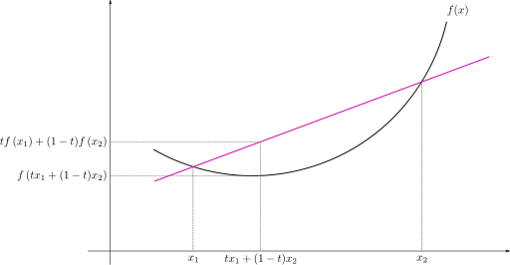
\includegraphics[scale=1.0]{fig8_13.png} 
\caption{볼록 함수와 젠센 부등식}
\label{fig:8-13}
\end{figure}

그림 \ref{fig:8-13}의 볼록 함수와 일차함수 사이의 관계로 젠센 부등식을 이해할 수 있다. $\varphi$가 볼록 함수일 때, 두 점 $x_1$과 $x_2$ 사이에서  $\varphi(x_1)$과 $\varphi(x_2)$의 가중치 평균(Weighted Average)을 나타내는 빨간색의 일차함수는 언제나 $\varphi$를 웃돈다. 수식 (\ref{eq:8-45})의 좌변이 $\varphi$를, 우변이 가중치 평균(각 $\varphi(x_{i})$의 가중치는 $a_{i}/\sum a_{i}$이다.)을 나타내므로 수식은 참임을 알 수 있다.  \\     

로그 함수는 오목 함수이다. 따라서 로그 우도에 대한 수식 (\ref{eq:8-42})에 젠센 부등식을 적용할 수 있도록 $q(Z)$를 도입해서 다음과 같이 나타내도록 하자. 단, $\sum_{Z} q(Z)=1$이여야 한다.  
\begin{equation}
\textrm{ln} L(\theta) =  \textrm{ln} (\sum_{Z} P(X, Z|\theta)) = \textrm{ln} (\sum_{Z} q(Z) \frac{P(X, Z|\theta))}{q(Z)} \label{eq:8-46}
\end{equation}
그러면 이제 젠슨 부등식의 $x_i$, $a_i$에 각각 $\frac{P(X, Z|\theta)}{q(Z)}$, $q(Z)$를 대입해서 다음의 식을 얻을 수 있다. 
\begin{equation}
\textrm{ln} L(\theta) =  \textrm{ln} (\sum_{Z} q(Z) \frac{P(X, Z|\theta)}{q(Z)}) \geq \sum_{Z} q(Z) \textrm{ln} \frac{P(X, Z|\theta)}{q(Z)} \label{eq:8-47}
\end{equation}
수식이 더 이상 등식이 아니게 된 것은 아쉽지만 이제는 식을 계속해서 전개해 나갈 수 있다.  
\begin{eqnarray}
\textrm{ln} L(\theta) & \geq & \sum_{Z} q(Z) \textrm{ln} \frac{P(X, Z|\theta)}{q(Z)} \nonumber  \\
& = & \sum_{Z} q(Z) \textrm{ln} P(X, Z|\theta) - q(Z) \textrm{ln} q(Z) \nonumber  \\
& = & E_{q(Z)} \textrm{ln} P(X, Z|\theta) + H(q)  \label{eq:8-48} 
\end{eqnarray}
여기서 함수 $H$는 Chapter 2에서 언급한 엔트로피(Entropy) 공식과 같으며, 구체적으로는 $H(X) = -\sum_{X} P(X=x) \textrm{ln} P(X=x)$를 의미한다. 다만, $H(q)$가 $q$에 대한 엔트로피 공식이라고 확실히 말할 수 있으려면 $q$가 정확히 확률 분포 함수여야 한다. 다시 말해, $q(Z) \geq 0$, $\sum_{Z} q(Z)=1$이 성립해야 한다. 이렇게 $q(Z)$가 확률 분포 함수가 된다면  수식 (\ref{eq:8-48})을 마지막까지 전개할 수 있게 된다. \\

%슬라이드 26
수식 (\ref{eq:8-48})의 결론을 하나의 함수로 나타내어보자.
\begin{equation}
Q(\theta, q) = E_{q(Z)} \textrm{ln} P(X, Z|\theta) + H(q) \label{eq:8-49}
\end{equation}
함수 $Q$는 임의의 확률 분포 함수 $q$에 대해서 $\textrm{ln} L(\theta) \geq Q(\theta, q)$를 만족시킨다. 따라서 $\textrm{ln} L(\theta)$의 하한값을 얻기 위해서는 $Q(\theta, q)$를 최대로 만드는 확률 분포 함수 $q$를 찾아야 한다. 이를 위해서 $Q(\theta, q)$를 다음과 같이 $\textrm{ln} L(\theta)$에 관한 식으로 전개하고, 혼란을 막기 위해서 따로 $L(\theta, q)$라고 부르겠다. 
\begin{eqnarray}
L(\theta, q) & = & \sum_{Z} q(Z) \textrm{ln} \frac{P(X, Z|\theta)}{q(Z)} \nonumber  \\
& = & \sum_{Z} q(Z) \textrm{ln} \frac{P(Z|X,\theta) P(X|\theta)}{q(Z)} \nonumber  \\
& = & \sum_{Z} (q(Z) \textrm{ln} \frac{P(Z|X,\theta)}{q(Z)} + q(Z) \textrm{ln} P(X|\theta))  \nonumber  \\
& = & \textrm{ln} P(X|\theta) + \sum_{Z} (q(Z) \textrm{ln} \frac{P(Z|X,\theta)}{q(Z)}) \nonumber  \\
& = & \textrm{ln} L(\theta) - \sum_{Z} (q(Z) \textrm{ln} \frac{q(Z)}{P(Z|X,\theta)}) \label{eq:8-50} 
\end{eqnarray}
수식 (\ref{eq:8-50})에 따르면 $\textrm{ln} L(\theta)$와 $L(\theta, q)$의 차이는 $\sum_{Z} (q(Z) \textrm{ln} \frac{q(Z)}{P(Z|X,\theta)})$에 의해서 결정된다. 따라서 다음을 최소화하면 $L(\theta, q)$가 $\textrm{ln} L(\theta)$에 최대 한도로 가까워진다. 
\begin{equation}
KL(q(Z) || P(Z|X,\theta)) = \sum_{Z} q(Z) \textrm{ln} \frac{q(Z)}{P(Z|X,\theta)} \label{eq:8-51}
\end{equation}
이러한 함수를 쿨백-라이블러 발산(Kullback–Leibler Divergence) 또는 줄여서 KL-발산(KL-Divergence)이라고 하며, 두 확률 분포 사이의 유사도를 확률 밀도 함수를 사용해서 측정하는 함수이다. KL-발산은 다음의 성질을 가진다. 먼저, 두 확률 밀도 함수 $P$, $Q$가 있을 때, $KL(P || Q) = \sum_{i} P(i) \textrm{ln} (P(i) / Q(i))$는 0보다 크거나 같다. 또한, $KL(P || Q)$가 0에 가까울수록 두 확률 변수는 유사점이 많으며, 만일 이것이 0이라면 $P$, $Q$는 정확히 일치한다고 할 수 있다. 마지막으로, $KL(P || Q)$와 $KL(Q || P)$는 일반적으로 다르기 때문에 이것은 두 확률 변수 사이의 비대칭(Non-Symmetric) 측정 함수이다. \\     

%슬라이드 27
\begin{figure}[ht] \centering 
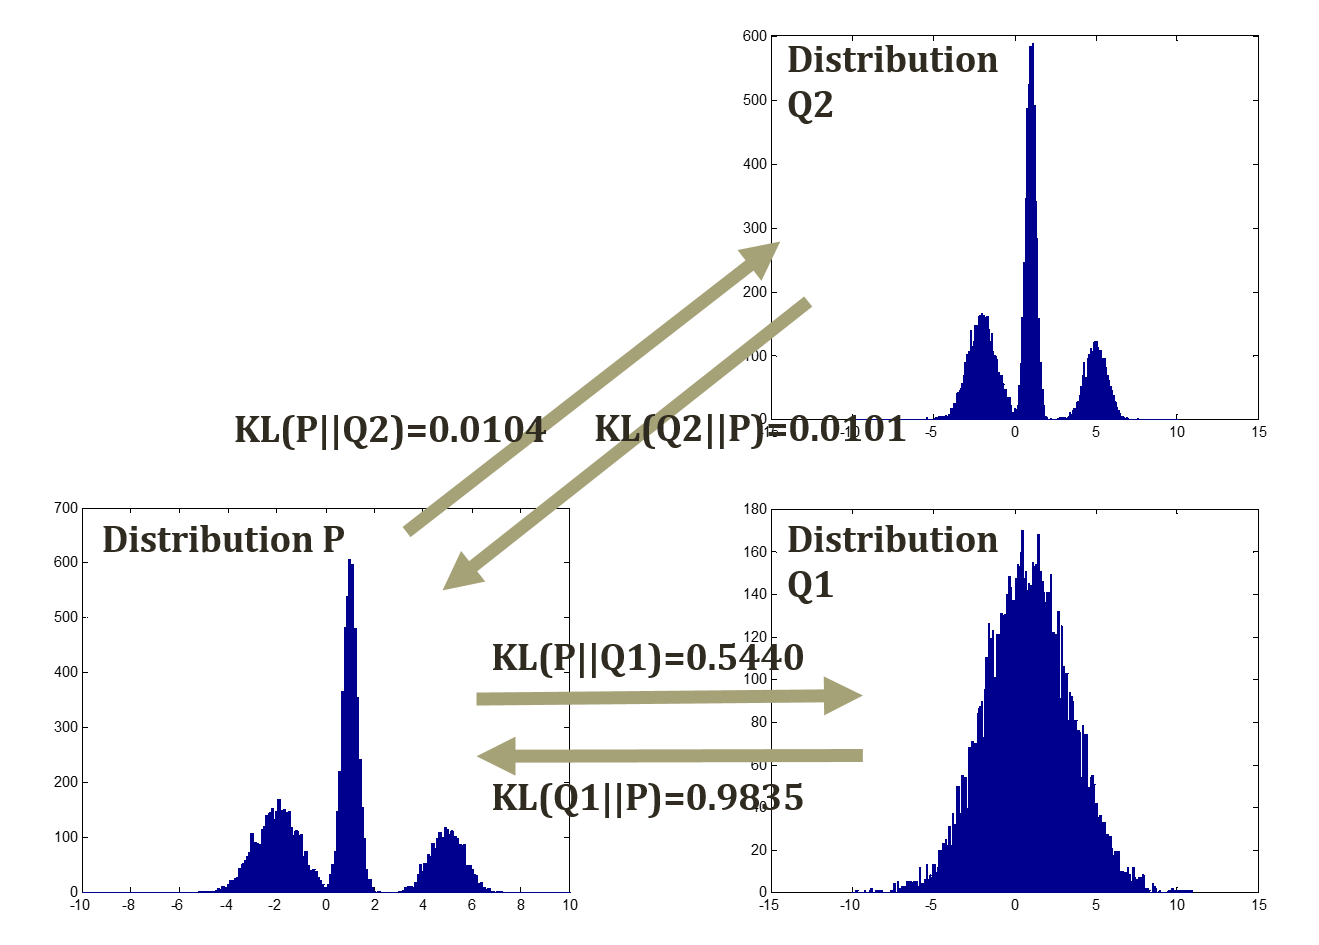
\includegraphics[scale=0.5]{fig8_14.png} 
\caption{KL-발산}
\label{fig:8-14}
\end{figure}

그림 \ref{fig:8-14}의 예시로 KL-발산을 이해해보자. 여기에는 $P$, $Q1$, $Q2$의 세 확률 변수에 대한 분포가 그래프로 표현되어 있다. 겉보기에 $P$와 $Q1$은 분포의 봉우리 개수가 각각 3개, 1개로써 크게 다른 분포라는 것을 느낄 수 있으며, 반대로 $P$와 $Q2$는 얼핏 보기에 분포의 형태가 상당히 비슷하다는 것을 알 수 있다. 그러나 이렇게 두 확률 변수가 같거나 다르다는 추측은 직관적인 느낌에 불과해 객관적이라고는 할 수 없으며, KL-발산으로 두 확률 변수가 얼마나 비슷한지를 지표로 확인할 수 있다. 그림 \ref{fig:8-14}의 확률 변수 사이의 KL-발산운 $KL(P || Q1)$과 $KL(Q1 || P)$가 각각 $0.5440$, $0.9835$, $KL(P || Q2)$와 $KL(Q2 || P)$는 각각 $0.0104$, $0.0101$로 나온다. 따라서 $P$와 $Q1$은 크게 다르지만 $P$와 $Q2$는 비슷하다는 것을 객관적으로 확인할 수가 있다. 한편, 같은 두 개의 확률 변수를 다룬 $KL(P || Q1)$과 $KL(Q1 || P)$의 값이 상당히 다르게 나오는데 이는 KL-발산의 비대칭성에 의한 것으로, $KL(P || Q1)$이 $P$의 입장에서 바라본 $Q1$과의 유사성을, $KL(Q1 || P)$은 $Q1$의 입장에서 바라본 $P$과의 유사성을 나타내기 때문이다. \\

%슬라이드 28
다시 본론으로 돌아가서, 수식 (\ref{eq:8-50})에 따르면 $L(\theta, q)$와 $\textrm{ln} L(\theta)$의 차이는 $KL(q(Z) || P(Z|X,\theta))$이다. 이것을 0으로 만들어주면, 다시 말해서 $q(Z)$를 $P(Z|X,\theta)$와 일치시킨다면, $L(\theta, q)$와 $\textrm{ln} L(\theta)$는 정확히 같게 된다. 따라서 시점 $t$에서 파라미터 $\theta$의 값을 $\theta^{t}$라고 한다면 이 때의 $q^{t}(Z)$는 $P(Z|X,\theta^t)$로 정하는 것이 최적이 된다. 다음은 $\theta^{t}$와 $q^{t}(Z)$를 $Q$에 대입한 것을 나타내며, 로그 우도 $\textrm{ln} L(\theta)$의 하한값이 된다.
\begin{equation}
Q(\theta^t, q^t) = E_{q^{t}(Z)} \textrm{ln} P(X, Z|\theta^t) + H(q^t) \label{eq:8-52}
\end{equation}
이제 새로이 갱신한 $q^t$에 대해서 더 이상 $\theta^{t}$가 최적이 아니므로 새로이 최적인 $\theta^{t+1}$를 찾아서 하한값을 높일 수가 있다. 그러한 $\theta^{t+1}$은 다음과 같이 나온다.  
\begin{equation}
\theta^{t+1} = \textrm{argmax}_{\theta} Q(\theta, q^t) = \textrm{argmax}_{\theta} E_{q^{t}(Z)} \textrm{ln} P(X, Z|\theta) \label{eq:8-53}
\end{equation}
이렇게 KL 발산을 활용해서 $\theta^{t}$에 대해서 최적인 $q^{t}(Z)$를 찾고, 이렇게 찾은 $q^{t}(Z)$에 대해서 다시 최적인 $\theta^{t+1}$을 찾아서 갱신해주는 과정의 반복이 바로 EM 알고리즘이 된다. \\

%슬라이드 29
\begin{figure}[ht] \centering 
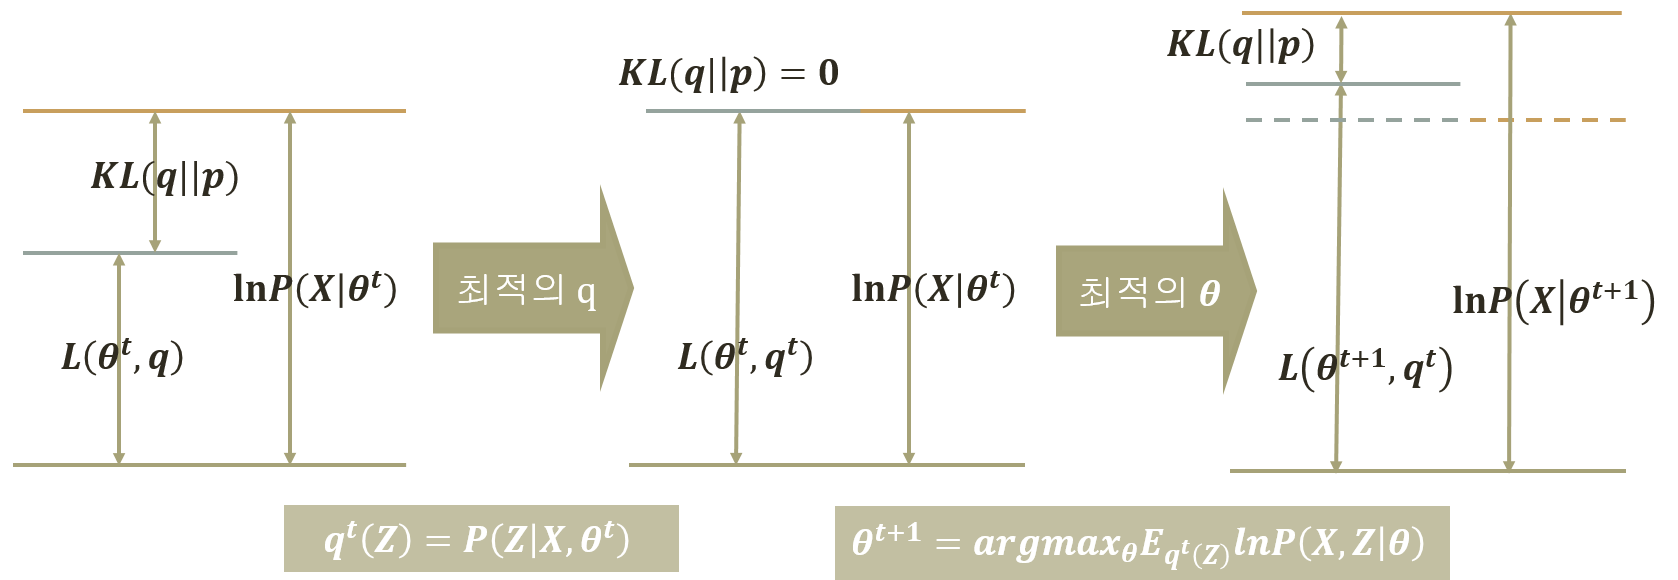
\includegraphics[scale=0.45]{fig8_15.png} 
\caption{EM 알고리즘의 반복}
\label{fig:8-15}
\end{figure}

이것을 알기 쉽게 그림으로 나타낸 것이 바로 그림 \ref{fig:8-15}이다. 처음에는 로그 우도 $\textrm{ln} L(\theta) = \textrm{ln} P(X|\theta)$는 $L(\theta, q)$와 $KL(q||p) = KL(q(Z) || P(Z|X,\theta))$의 합으로 이루어져 있다. 여기서 두 번째 그림에서처럼 $q(Z)$를 $P(Z|X,\theta^{t})$와 일치시키면 $KL(q||p)=0$이 되어 $L(\theta^{t}, q)$는 최대가 되며, 이 때의 $q$를 $q^{t}$로 둘 수가 있다. 이제 세 번째 그림에서처럼 $q^{t}$가 주어진 상황에서 $\theta$값을 다시 갱신해서 $L(\theta, q^{t})$가 최대가 되도록 하자. 그러면 $p$ 또한 변하므로 $KL(q||p)$는 다시 0이 아니게 된다. 따라서 처음 과정으로 돌아가서 $KL(q||p)$을 0으로 만들어주는 $q$를 찾아야 한다.       

\begin{figure}[ht] \centering 
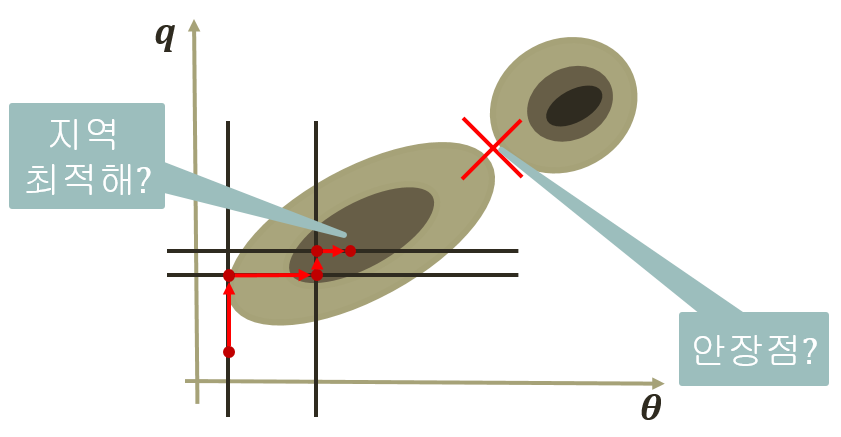
\includegraphics[scale=0.8]{fig8_16.png} 
\caption{EM 알고리즘을 통한 최적해의 탐색}
\label{fig:8-16}
\end{figure}

이처럼 EM 알고리즘은 잠재 변수의 확률 분포 $q$와 파라미터 $\theta$를 바꿔주는 과정을 계속해서 반복하면서 최대 로그 우도값을 찾는 과정이다. 그림 \ref{fig:8-16}에서 이러한 EM 알고리즘의 과정을 최적해를 탐색하는 관점으로 묘사하였다. 그림에서는 서남쪽의 지점에서부터 시작해서 $q$를 갱신하면서 북쪽으로 이동하고, $\theta$를 갱신하면서 동쪽으로 이동하면서 계속해서 최적해를 향하여 올라가는 것이 나타나 있다. 그러나 여기에는 초기 시작 지점에 따라서 지역 최적해에 빠질 우려가 있다. 예를 들어, 그림 \ref{fig:8-16}에서처럼 동북쪽에 전역 최적해가 따로 있음에도 불구하고 마지막에는 중앙에 있는 지역 최적해에 머물게 된다. 여기에 더해서 해가 지역 최적해조차 아닌 안장점(Saddle Point)에 빠질 위험도 있다. 하지만 이러한 문제점에도 불구하고 EM 알고리즘은 현실에서 상당히 잘 작동하며, 많은 자율 학습 모델에서 쓰이고 있다. \\

%슬라이드 30, 31
마지막으로 EM 알고리즘의 과정을 정리해보자. 먼저, 파라미터 $\theta$의 초기값을 임의로 $\theta^0$로 정해준다. 그리고 다음의 기댓값 과정과 최대화 과정을 반복한다. 먼저 기댓값 과정은 $\theta^t$가 있을 때, $L(\theta^t, q)$를 최대로 만드는 $q = q^t(Z)=P(Z|X, \theta^t)$를 정해주는 과정이다. 다음으로 최대화 과정은 $q^t$가 있을 때, $Q(\theta, q^t)$를 최대로 만드는 $\theta^{t+1}$을 찾는 과정이다. 여기서는 잠재 변수인 $Z$의 확률 분포가 고정되어 있으므로, 기존의 방법대로 우도를 최대화하는 최우추정값을 찾는 과정을 수행하면 된다. EM 알고리즘을 활용한다면 잠재 변수에 대한 최적의 할당을 찾을 수 있으며, 우리는 k-평균 모델과 가우시안 혼합 모델에서 최적의 군집화를 위해 EM 알고리즘을 사용하였다.  


\end{document}
